%!TEX program = xelatex
%!TEX options=--shell-escape
\documentclass[12pt]{article}

%
\usepackage[scheme=plain]{ctex}
%
\usepackage{fontspec}
%
\usepackage[margin = 1in]{geometry}

%
\usepackage[dvipsnames]{xcolor}
\usepackage[many]{tcolorbox}

%
\usepackage{amsmath}
\usepackage{amssymb}
\usepackage{amsthm}
%
\usepackage{tensor}
%
\usepackage{slashed}
\usepackage{physics}
\usepackage{simpler-wick}

%
\usepackage{mathtools}

%
\usepackage{bm}
\newcommand{\dbar}{\dif\hspace*{-0.18em}\bar{}\hspace*{0.2em}}
\DeclareMathAlphabet\mathbfcal{OMS}{cmsy}{b}{n}
%\usepackage{bbold}
\newcommand*{\dif}{\mathop{}\!\mathrm{d}}
\newcommand*{\euler}{\mathrm{e}}
\newcommand*{\imagi}{\mathrm{i}}

\renewcommand{\vec}[1]{\boldsymbol{\mathbf{#1}}}

\usepackage{caption}
\usepackage{multirow}
\usepackage{enumitem}

%
\usepackage{mathrsfs}
\usepackage{dsfont}

%
\usepackage{hyperref}
\hypersetup{
    colorlinks=true,
    linkcolor=violet,
    filecolor=blue,
    urlcolor=blue,
    citecolor=cyan,
}

%
\usepackage{graphicx}
\usepackage{subfig}
%
\graphicspath{{../figures/}}

\usepackage{tikz}
\usetikzlibrary{positioning}
\usetikzlibrary{calc}

\usepackage{listings}
\usepackage{lstautogobble}
\lstset{
    basicstyle=\ttfamily,
    columns=fullflexible,
    autogobble=true,
}

%
\usepackage{indentfirst}
%
\setlength{\parindent}{2em}
\linespread{1.25}

%
% \setmainfont{Times New Roman}

\title{Note}
\author{Feng-Yang Hsieh}
\date{}

\begin{document}
\maketitle

\section{Higgs Production}% (fold)
\label{sec:higgs_production}
    We aim to apply deep learning methods to distinguish vector boson fusion (VBF) from gluon-gluon fusion (GGF) and Higgs production at the Large Hadron Collider (LHC).

    We aim to apply the CWoLa method, enabling us to utilize real data without prior knowledge of the true label.
% section higgs_production (end)
\section{Sample Preparation}% (fold)
\label{sec:sample_preparation}
    \subsection{Monte Carlo samples}% (fold)
    \label{sub:monte_carlo_samples}
        We consider Standard Model (SM) di-photon Higgs events produced via GGF and VBF channels at a center-of-mass energy of $\sqrt{s} = 14$ TeV. The Higgs boson events are generated using \verb|MadGraph 3.3.1|~\cite{Alwall:2014hca} for both GGF and VBF production. The Higgs decays into the di-photon final state, and the parton showering and hadronization are simulated using \verb|Pythia 8.306|~\cite{Sjostrand:2014zea}. The detector simulation is conducted by \verb|Delphes 3.4.2|~\cite{deFavereau:2013fsa}. Jet reconstruction is performed using \verb|FastJet 3.3.2|~\cite{Cacciari:2011ma} with the anti-$k_t$ algorithm~\cite{Cacciari:2008gp} and a jet radius of $R = 0.4$. These jets are required to have transverse momentum $p_{\text{T}} > 25$ GeV.

        The following \verb|MadGraph| scripts generate Monte Carlo samples for each production channel.
        \paragraph{GGF Higgs Sample Generation}
        \begin{lstlisting}
            generate p p > h QCD<=99 [QCD]
            output GGF_Higgs
            launch GGF_Higgs

            shower=Pythia8
            detector=Delphes
            analysis=OFF
            madspin=OFF
            done

            set run_card nevents 100000
            set run_card ebeam1 7000.0
            set run_card ebeam2 7000.0

            set run_card use_syst False

            set pythia8_card 25:onMode = off
            set pythia8_card 25:onIfMatch = 22 22
            done
        \end{lstlisting}
        \paragraph{VBF Higgs Sample Generation}
        \begin{lstlisting}
            define v = w+ w- z
            generate p p > h j j $$v
            output VBF_Higgs
            launch VBF_Higgs

            shower=Pythia8
            detector=Delphes
            analysis=OFF
            madspin=OFF
            done

            set run_card nevents 100000
            set run_card ebeam1 7000.0
            set run_card ebeam2 7000.0

            set run_card use_syst False

            set pythia8_card 25:onMode = off
            set pythia8_card 25:onIfMatch = 22 22
            done
        \end{lstlisting}
    % subsection monte_carlo_samples (end)
    \subsection{Event selection}% (fold)
    \label{sub:event_selection}
        The selection cuts after the \verb|Delphes| simulation:
        \begin{itemize}
            \item $n_{\gamma}$ cut: The number of photons should be at least 2.
            \item $n_{j}$ cut: The number of jets should be at least 2.
            \item $m_{\gamma\gamma}$ cut: The invariant mass of two leading photons $m_{\gamma\gamma}$ are required $\text{120 GeV} \le m_{\gamma\gamma} \le \text{130 GeV}$.
        \end{itemize}

        Table~\ref{tab:GGF_VBF_Higgs_cutflow_number} summarizes the cutflow number at different selection cuts.
        \begin{table}[htpb]
            \centering
            \caption{Number of passing events and passing rates for GGF and VBF Higgs production at different selection cuts.}
            \label{tab:GGF_VBF_Higgs_cutflow_number}
            \begin{tabular}{l|rr|rr}
                Cut                    & GGF    & pass rate & VBF    & pass rate \\ \hline
                Total                  & 100000 & 1         & 100000 & 1         \\
                $n_{\gamma}$ cut       & 48286  & 0.48      & 53087  & 0.53      \\
                $n_j$ cut              & 9302   & 0.09      & 42860  & 0.43      \\
                $m_{\gamma\gamma}$ cut & 8864   & 0.09      & 40694  & 0.41     
            \end{tabular}
        \end{table}
        
        Figure~\ref{fig:mjj_deta_distribution} shows the distributions of $m_{jj}$ (the invariant mass of the two leading jets) and $\Delta\eta_{jj}$ (the pseudorapidity difference between the two leading jets). The scatter plot of $m_{jj}$ versus $\Delta\eta_{jj}$ is presented in Figure~\ref{fig:mjj_deta_scatter}.
        \begin{figure}[htpb]
            \centering
            \subfloat[$m_{jj}$ distribution]{
                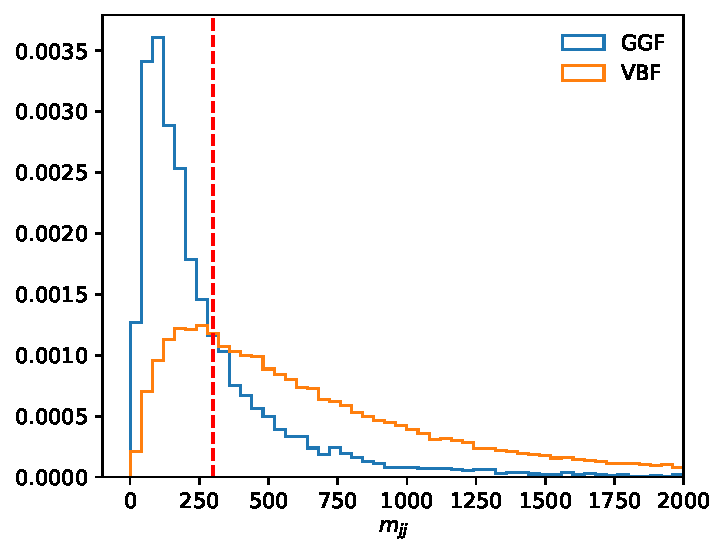
\includegraphics[width=0.45\textwidth]{mjj_distribution.pdf}
            }
            \subfloat[$\Delta\eta_{jj}$ distribution]{
                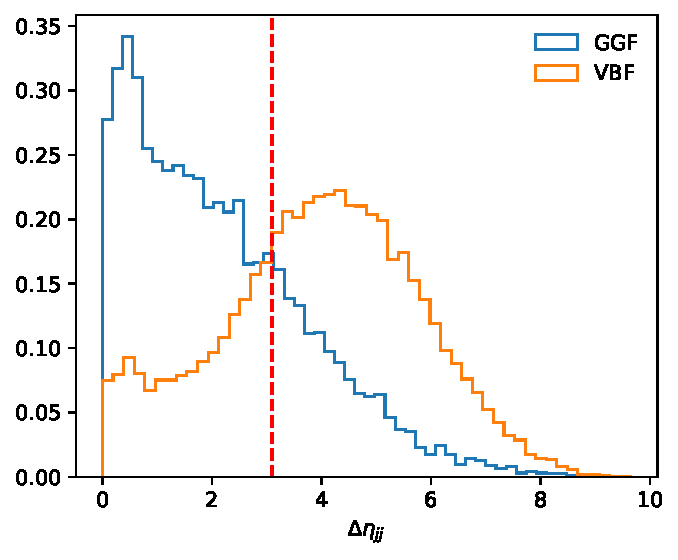
\includegraphics[width=0.45\textwidth]{deta_distribution.pdf}
            }
            \caption{Distributions of the invariant mass $m_{jj}$ and pseudorapidity difference $\Delta\eta_{jj}$ of the two leading jets. Red dashed lines are selection cuts used to construct mixed datasets.}
            \label{fig:mjj_deta_distribution}
        \end{figure}
        \begin{figure}[htpb]
            \centering
            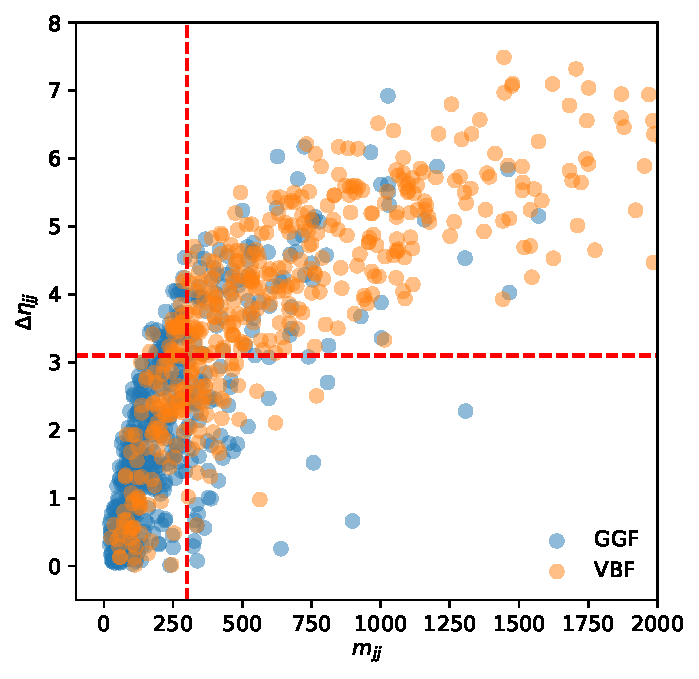
\includegraphics[width=0.45\textwidth]{mjj_deta_scatter_plot.pdf}
            \caption{Scatter plot of $m_{jj}$ versus $\Delta\eta_{jj}$. Red dashed lines are selection cuts used to construct mixed datasets.}
            \label{fig:mjj_deta_scatter}
        \end{figure}
    % subsection event_selection (end)
    \subsection{Event image}% (fold)
    \label{sub:event_image}
        The inputs for the neural networks are event images~\cite{Kasieczka:2019dbj,deOliveira:2015xxd, Kasieczka2017nv}. These images are constructed from events that pass the kinematic selection criteria described in section~\ref{sub:event_selection}. Each event image has three channels corresponding to calorimeter towers, tracks, and photons. The following preprocessing steps are applied to all event constituents:
        \begin{enumerate}
            \item Translation: Compute the $p_{\text{T}}$-weighted center in the $\phi$ coordinates, then shift this point to the origin.
            \item Flipping: Flip the highest $p_{\text{T}}$ quadrant to the first quadrant.
            \item Pixelation: Pixelate in a $\eta \in [-5, 5],\ \phi \in [-\pi, \pi]$ box, with $40 \times 40$ pixels 
        \end{enumerate}

        Figure~\ref{fig:GGF_VEF_event_image} shows the event images for GGF and VBF production modes.
        \begin{figure}[htpb]
            \centering
            \subfloat[GGF: Calorimeter Tower]{
                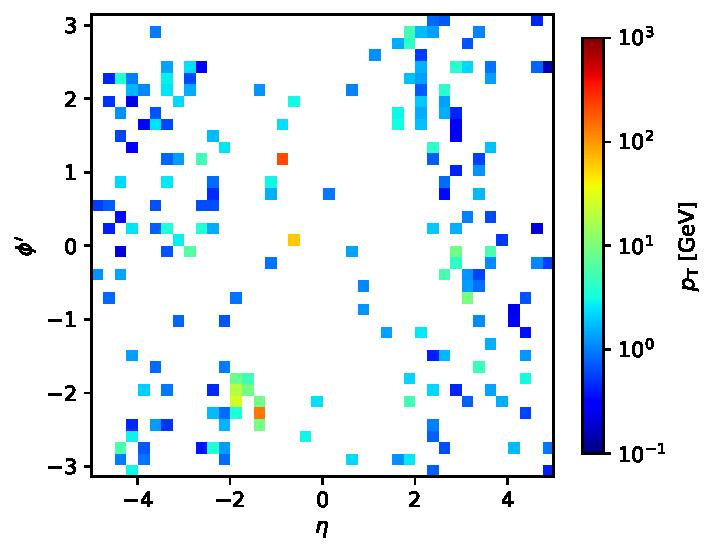
\includegraphics[width=0.45\textwidth]{event_image_GGF-tower.pdf}
            }
            \subfloat[VBF: Calorimeter Tower]{
                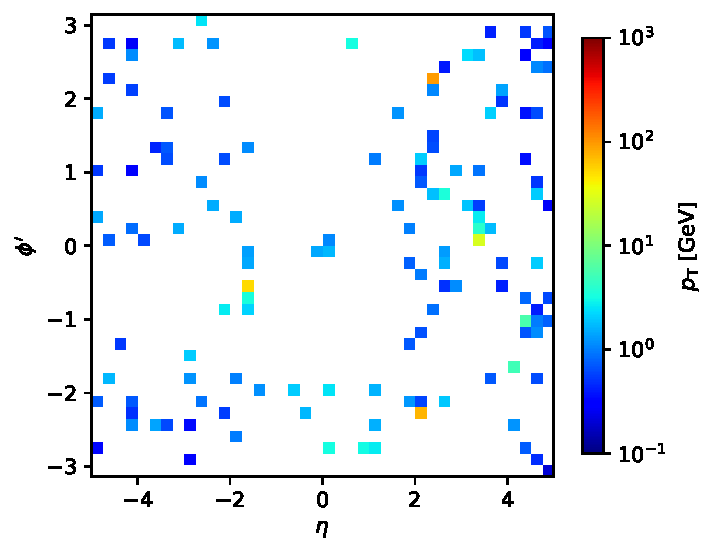
\includegraphics[width=0.45\textwidth]{event_image_VBF-tower.pdf}
            } \\
            \subfloat[GGF: Track]{
                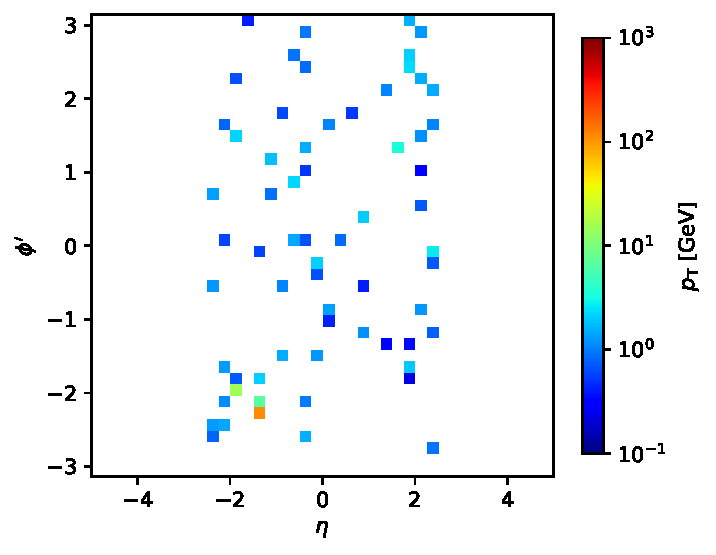
\includegraphics[width=0.45\textwidth]{event_image_GGF-track.pdf}
            }
            \subfloat[VBF: Track]{
                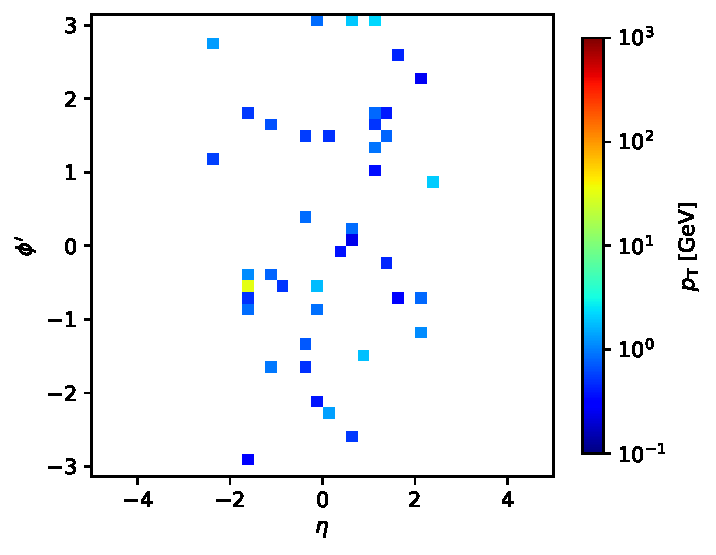
\includegraphics[width=0.45\textwidth]{event_image_VBF-track.pdf}
            } \\
            \subfloat[GGF: Photon]{
                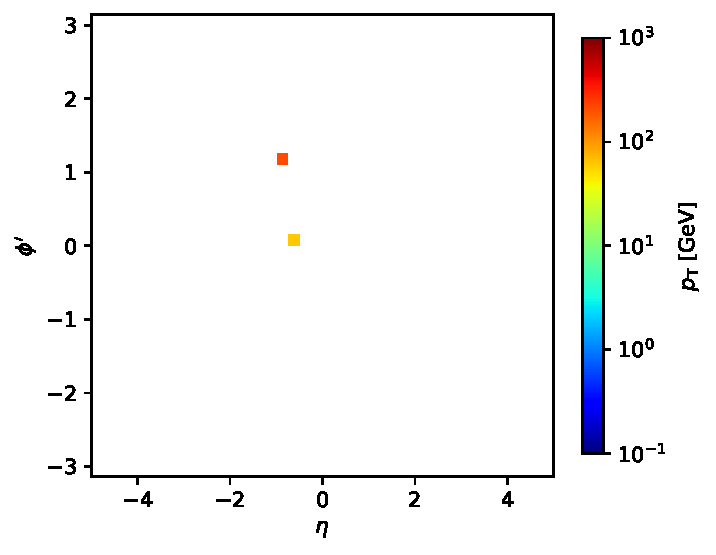
\includegraphics[width=0.45\textwidth]{event_image_GGF-photon.pdf}
            }
            \subfloat[VBF: Photon]{
                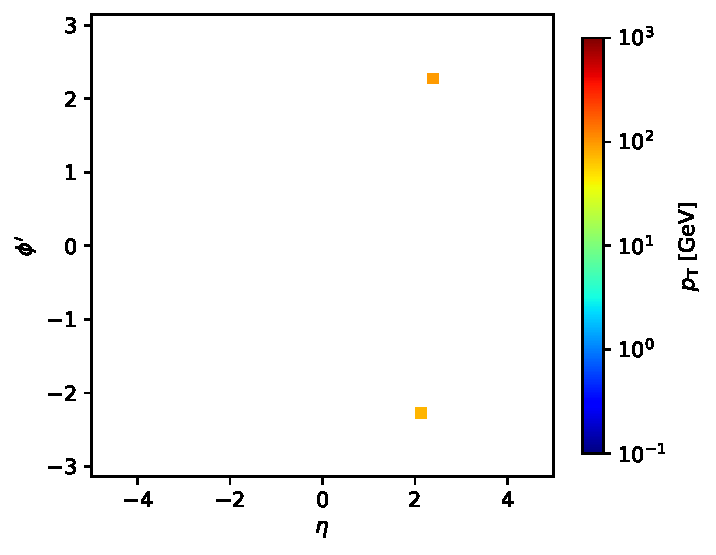
\includegraphics[width=0.45\textwidth]{event_image_VBF-photon.pdf}
            }
            \caption{Event images for GGF and VBF production, separately shown for calorimeter towers, tracks, and photons.}
            \label{fig:GGF_VEF_event_image}
        \end{figure}
    % subsection event_image (end)
    \subsection{Mixed datasets}% (fold)
    \label{sub:mixed_datasets}
        Based on figure~\ref{fig:mjj_deta_distribution}, we set selection cuts of $m_{jj} > 300$ GeV and $\Delta\eta_{jj} > 3.1$. We consider three cases: applying each cut individually and simultaneously. These cuts define the signal region (SR), which is VBF-like, and the background region (BR), which is GGF-like. Table~\ref{tab:GGF_VBF_Higgs_cutflow_number_mixed_dataset} summarizes the cutflow results for different selection criteria.
        \begin{table}[htpb]
            \centering
            \caption{Number of passing events and passing rates for GGF and VBF Higgs production under different selection cuts.}
            \label{tab:GGF_VBF_Higgs_cutflow_number_mixed_dataset}
            \begin{tabular}{l|rr|rr}
                Cut                                & GGF    & pass rate & VBF    & pass rate \\ \hline
                Total                              & 100000 & 1.00      & 100000 & 1.00      \\
                $n_{\gamma}$ cut                   & 9302   & 0.09      & 42860  & 0.43      \\
                $n_j$ cut                          & 9302   & 0.09      & 42860  & 0.43      \\
                $m_{\gamma\gamma}$ cut             & 8864   & 0.09      & 40694  & 0.41      \\ \hline
                $m_{jj}$ cut: SR                   & 2695   & 0.03      & 29496  & 0.29      \\
                $m_{jj}$ cut: BR                   & 6169   & 0.06      & 11198  & 0.11      \\ \hline
                $\Delta\eta_{jj}$ cut: SR          & 2317   & 0.02      & 28160  & 0.28      \\
                $\Delta\eta_{jj}$ cut: BR          & 6547   & 0.07      & 12534  & 0.13      \\ \hline
                $m_{jj}, \Delta\eta_{jj}$ cuts: SR & 1832   & 0.02      & 26446  & 0.26      \\
                $m_{jj}, \Delta\eta_{jj}$ cuts: BR & 5684   & 0.06      & 9484   & 0.09     
            \end{tabular}
        \end{table}

        The total cross-section for VBF production is $\sigma_{\text{VBF}} = 4.278$ pb$^{-1}$ at NNLO and for GGF production is $\sigma_{\text{GGF}} = 54.67$ pb$^{-1}$ at N3LO, as referenced in \href{https://twiki.cern.ch/twiki/bin/view/LHCPhysics/CERNYellowReportPageAt14TeV}{this link}. The branching ratio for the di-photon decay channel is $\Gamma\left( h \to \gamma\gamma \right) = 2.270 \times 10^{-3}$, as given in \href{https://twiki.cern.ch/twiki/bin/view/LHCPhysics/CERNYellowReportPageBR}{this link}.

        Assuming the luminosity of $\mathcal{L} = \text{300 fb}^{-1}$, we can estimate the number of events belonging to the SR and BR. These results are summarized in table~\ref{tab:number_of_event_in_mixed_dataset}.
        \begin{table}[htpb]
            \centering
            \caption{The number of events of mixed datasets under different selection cuts.}
            \label{tab:number_of_event_in_mixed_dataset}
            \subfloat[$m_{jj} > 300$ GeV]{
                \begin{tabular}{c|cc}
                       & GGF & VBF \\ \hline
                    BR & 2297 & 326 \\
                    SR & 1003 & 859
                \end{tabular}
            }
            \subfloat[$\Delta\eta_{jj} > 3.1$]{
                \begin{tabular}{c|cc}
                       & GGF & VBF \\ \hline
                    BR & 2437 & 365 \\
                    SR & 863  & 820
                \end{tabular}
            } \\
            \subfloat[$m_{jj} > 300$ GeV, \newline $\Delta\eta_{jj} > 3.1$]{
                \begin{tabular}{c|cc}
                       & GGF & VBF \\ \hline
                    BR & 2116 & 276 \\
                    SR & 682  & 770
                \end{tabular}
            }
        \end{table}
    % subsection mixed_datasets (end)
% section sample_preparation (end)
\section{Training CNN}% (fold)
\label{sec:training_cnn}
    The total sample sizes are mentioned in section~\ref{sub:mixed_datasets}. We allocate 80\% of the data for training and 20\% for validation. The testing set consists of the SR's 10,000 VBF and 10,000 GGF events.

    The convolutional neural network (CNN) model structure is summarized in figure~\ref{fig:cnn_model_structure}. The internal node uses the rectified linear unit (ReLU) as the activation function. The loss function is the binary cross-entropy. The \verb|Adam| optimizer minimizes the loss value. The learning rate is $10^{-4}$, and the batch size is 512. We employ the early stopping technique to prevent over-training issues with patience of 10.
    \begin{figure}[htpb]
        \centering
        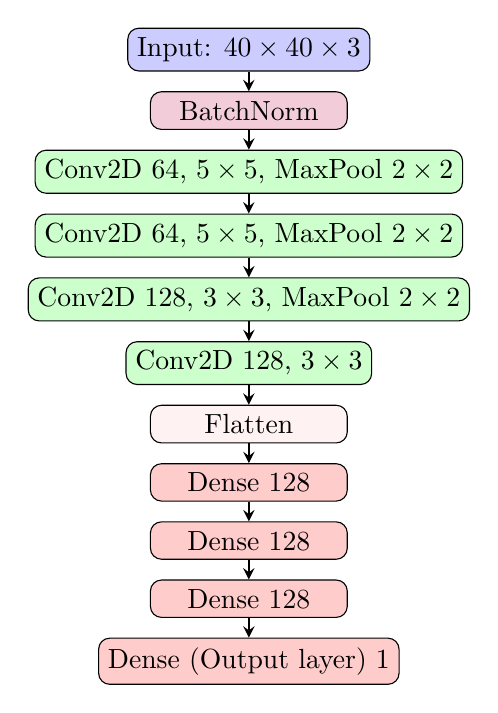
\begin{tikzpicture}[
            layer/.style={draw, rounded corners, minimum width=2.5cm, text centered},
            arrow/.style={-stealth, thick},
            node distance=0.25cm,
        ]
        % Input layer
        \node (input) [layer, fill=blue!20,] {Input: $40 \times 40 \times 3$};

        % Jet 1 layers
        \node (bn1) [below=of input, layer, fill=purple!20] {BatchNorm};


        % Conv1_1 layer positioned between bn1 and bn2
        \node (conv1_1) [below=0.25cm of bn1, layer, fill=green!20] {Conv2D 64, $5 \times 5$, MaxPool $2 \times 2$};

        % Other Conv layers
        \node (conv2_1) [below=of conv1_1, layer, fill=green!20] {Conv2D 64, $5 \times 5$, MaxPool $2 \times 2$};
        \node (conv3_1) [below=of conv2_1, layer, fill=green!20] {Conv2D 128, $3 \times 3$, MaxPool $2 \times 2$};
        \node (conv4_1) [below=of conv3_1, layer, fill=green!20] {Conv2D 128, $3 \times 3$};

        % Dense layers
        \node (flatten1) [below=of conv4_1, layer, fill=pink!20] {Flatten};
        \node (dense1_1) [below=of flatten1, layer, fill=red!20] {Dense 128};
        \node (dense2_1) [below=of dense1_1, layer, fill=red!20] {Dense 128};
        \node (dense3_1) [below=of dense2_1, layer, fill=red!20] {Dense 128};
        \node (output1) [below=of dense3_1, layer, fill=red!20] {Dense (Output layer) 1};


        % Arrows for BN
        \draw [arrow] (input) -- (bn1);
        \draw [arrow] (bn1) -- (conv1_1);
        \draw [arrow] (conv1_1) -- (conv2_1);
        \draw [arrow] (conv2_1) -- (conv3_1);
        \draw [arrow] (conv3_1) -- (conv4_1);
        \draw [arrow] (conv4_1) -- (flatten1);
        \draw [arrow] (flatten1) -- (dense1_1);
        \draw [arrow] (dense1_1) -- (dense2_1);
        \draw [arrow] (dense2_1) -- (dense3_1);
        \draw [arrow] (dense3_1) -- (output1);

        \end{tikzpicture}
        \caption{The architecture of the CNN model with key hyperparameters.}
        \label{fig:cnn_model_structure}
    \end{figure}

    The training results are summarized in table~\ref{tab:CWoLa_CNN_training_results}. The performance of the $\Delta\eta_{jj}$ cuts is better than the $m_{jj}$ cut. Moreover, when both cuts are applied together, the performance is slightly worse than when applying either cut individually.
    \begin{table}[htpb]
        \centering
        \caption{The CNN training results. The ACC and AUC are evaluated based on 10 training. The selection cuts of $m_{jj} > \text{300 GeV}$ and $\Delta\eta_{jj} > 3.1$ are applied.}
        \label{tab:CWoLa_CNN_training_results}
        \begin{tabular}{l|cc|cc}
                                      & \multicolumn{2}{c|}{$M_1 / M_2$}      & \multicolumn{2}{c}{$S / B$}           \\ \hline
            Cut                       & ACC               & AUC               & ACC               & AUC               \\ \hline
            $m_{jj}$                  & $0.712 \pm 0.023$ & $0.741 \pm 0.041$ & $0.576 \pm 0.010$ & $0.596 \pm 0.014$ \\
            $\Delta\eta_{jj}$         & $0.828 \pm 0.043$ & $0.889 \pm 0.050$ & $0.604 \pm 0.014$ & $0.630 \pm 0.015$ \\
            $m_{jj}, \Delta\eta_{jj}$ & $0.753 \pm 0.022$ & $0.792 \pm 0.035$ & $0.573 \pm 0.007$ & $0.596 \pm 0.008$
        \end{tabular}
    \end{table}
    % subsection training_cnn (end)
    \subsection{More events}% (fold)
    \label{sub:more_events}
        This section assumes the luminosity of $\mathcal{L} = \text{3000 fb}^{-1}$. The number of events belonging to the SR and BR are summarized in table~\ref{tab:number_of_event_in_mixed_dataset_3000}.
        \begin{table}[htpb]
            \centering
            \caption{The number of events of mixed datasets under different selection cuts.}
            \label{tab:number_of_event_in_mixed_dataset_3000}
            \subfloat[$m_{jj} > 300$ GeV]{
                \begin{tabular}{c|cc}
                       & GGF & VBF \\ \hline
                    BR & 22967 & 3262 \\
                    SR & 10034 & 8593
                \end{tabular}
            }
            \subfloat[$\Delta\eta_{jj} > 3.1$]{
                \begin{tabular}{c|cc}
                       & GGF & VBF \\ \hline
                    BR & 24375 & 3652 \\
                    SR & 8626  & 8204
                \end{tabular}
            } \\
            \subfloat[$m_{jj} > 300$ GeV, \newline $\Delta\eta_{jj} > 3.1$]{
                \begin{tabular}{c|cc}
                       & GGF & VBF \\ \hline
                    BR & 21162 & 2763 \\
                    SR & 6821  & 7705
                \end{tabular}
            }
        \end{table}

        The training results are summarized in table~\ref{tab:CWoLa_CNN_training_results_3000}. All datasets' performance is better than the results in table~\ref{tab:CWoLa_CNN_training_results}. The $\Delta\eta_{jj}$ cut performs better than the $m_{jj}$ cut. Moreover, when both cuts are applied together, the performance is slightly worse than the $\Delta\eta_{jj}$ cut but better than $m_{jj}$. These results are similar to the previous one. 
        \begin{table}[htpb]
            \centering
            \caption{The CNN training results. The ACC and AUC are evaluated based on 10 training. The selection cuts of $m_{jj} > \text{300 GeV}$ and $\Delta\eta_{jj} > 3.1$ are applied.}
            \label{tab:CWoLa_CNN_training_results_3000}
            \begin{tabular}{l|cc|cc}
                                          & \multicolumn{2}{c|}{$M_1 / M_2$}      & \multicolumn{2}{c}{$S / B$}           \\ \hline
                Cut                       & ACC               & AUC               & ACC               & AUC               \\ \hline
                $m_{jj}$                  & $0.907 \pm 0.002$ & $0.969 \pm 0.002$ & $0.598 \pm 0.008$ & $0.625 \pm 0.009$ \\
                $\Delta\eta_{jj}$         & $0.931 \pm 0.004$ & $0.979 \pm 0.002$ & $0.615 \pm 0.005$ & $0.648 \pm 0.006$ \\
                $m_{jj}, \Delta\eta_{jj}$ & $0.929 \pm 0.003$ & $0.978 \pm 0.002$ & $0.608 \pm 0.004$ & $0.638 \pm 0.005$
            \end{tabular}
        \end{table}
    % subsection more_events (end)
% section training_cnn (end)
\section{\texorpdfstring{$p_{\mathrm{T}}$}{pT} normalization}% (fold)
\label{sec:pt_normalization}
    
    To remove the potential dependence of the input samples on $m_{jj}$, we standardize the event images to remove the difference in input data distributions between the SR and BR. We calculate the mean and standard deviation of the event image transverse momentum and use these values to standardize each event image. We standardize each channel separately.
    
    The number of events in the SR and BR are the same as previously in table~\ref{tab:number_of_event_in_mixed_dataset_3000}.

    The training results are summarized in table~\ref{tab:CWoLa_CNN_training_results_3000_pT_norm}. The $m_{jj}$ cut performs better than the previous one (table~\ref{tab:CWoLa_CNN_training_results_3000}). 
    \begin{table}[htpb]
        \centering
        \caption{The CNN training results with $p_{\text{T}}$ normalization technique. The ACC and AUC are evaluated based on 10 training. The selection cuts of $m_{jj} > \text{300 GeV}$ and $\Delta\eta_{jj} > 3.1$ are applied. }
        \label{tab:CWoLa_CNN_training_results_3000_pT_norm}
        \begin{tabular}{l|cc|cc}
                                      & \multicolumn{2}{c|}{$M_1 / M_2$}      & \multicolumn{2}{c}{$S / B$}           \\ \hline
            Cut                       & ACC               & AUC               & ACC               & AUC               \\ \hline
            $m_{jj}$                  & $0.874 \pm 0.004$ & $0.946 \pm 0.003$ & $0.624 \pm 0.005$ & $0.663 \pm 0.006$ \\
            $\Delta\eta_{jj}$         & $0.928 \pm 0.005$ & $0.979 \pm 0.002$ & $0.597 \pm 0.005$ & $0.630 \pm 0.006$ \\
            $m_{jj}, \Delta\eta_{jj}$ & $0.917 \pm 0.003$ & $0.973 \pm 0.002$ & $0.603 \pm 0.004$ & $0.636 \pm 0.006$
        \end{tabular}
    \end{table}

% section pt_normalization (end)
\section{Different cut setting}% (fold)
\label{sec:different_cut_setting}
    
    We set selection cuts of $m_{jj} > 225$ GeV and $\Delta\eta_{jj} > 2.3$ to ensure the SR and BR datasets have similar sizes. Table~\ref{tab:GGF_VBF_Higgs_cutflow_number_mixed_dataset_225_2.3} summarizes the cutflow results for different selection criteria.
    \begin{table}[htpb]
        \centering
        \caption{Number of passing events and passing rates for GGF and VBF Higgs production under different selection cuts.}
        \label{tab:GGF_VBF_Higgs_cutflow_number_mixed_dataset_225_2.3}
        \begin{tabular}{l|rr|rr}
            Cut                                & GGF    & pass rate & VBF    & pass rate \\ \hline
            Total                              & 100000 & 1.00      & 100000 & 1.00      \\
            $n_{\gamma}$ cut                   & 9302   & 0.09      & 42860  & 0.43      \\
            $n_j$ cut                          & 9302   & 0.09      & 42860  & 0.43      \\
            $m_{\gamma\gamma}$ cut             & 8864   & 0.09      & 40694  & 0.41      \\ \hline
            $m_{jj}$ cut: SR                   & 3638   & 0.04      & 32993  & 0.33      \\
            $m_{jj}$ cut: BR                   & 5226   & 0.05      & 7701   & 0.08      \\ \hline
            $\Delta\eta_{jj}$ cut: SR          & 3611   & 0.04      & 32914  & 0.33      \\
            $\Delta\eta_{jj}$ cut: BR          & 5253   & 0.05      & 7780   & 0.08      \\ \hline
            $m_{jj}, \Delta\eta_{jj}$ cuts: SR & 2842   & 0.03      & 31113  & 0.31      \\
            $m_{jj}, \Delta\eta_{jj}$ cuts: BR & 4457   & 0.04      & 5900   & 0.06     
        \end{tabular}
    \end{table}

    Assuming the luminosity of $\mathcal{L} = \text{3000 fb}^{-1}$, we can estimate the number of events belonging to the SR and BR. These results are summarized in table~\ref{tab:number_of_event_in_mixed_dataset_225_2.3}
    \begin{table}[htpb]
        \centering
        \caption{The number of events of mixed datasets under different selection cuts.}
        \label{tab:number_of_event_in_mixed_dataset_225_2.3}
        \subfloat[$m_{jj} > 225$ GeV]{
            \begin{tabular}{c|cc}
                   & GGF & VBF \\ \hline
                BR & 19457 & 2244 \\
                SR & 13544 & 9612
            \end{tabular}
        }
        \subfloat[$\Delta\eta_{jj} > 2.3$]{
            \begin{tabular}{c|cc}
                   & GGF & VBF \\ \hline
                BR & 19557 & 2267 \\
                SR & 13444 & 9589
            \end{tabular}
        } \\
        \subfloat[$m_{jj} > 225$ GeV, \newline $\Delta\eta_{jj} > 2.3$]{
            \begin{tabular}{c|cc}
                   & GGF & VBF \\ \hline
                BR & 16594 & 1719 \\
                SR & 10581 & 9064
            \end{tabular}
        }
    \end{table}

    The training results are summarized in table~\ref{tab:CWoLa_CNN_training_results_3000_pT_norm_225_2.3}. The results are better than the table~\ref{tab:CWoLa_CNN_training_results_3000_pT_norm} by 1\%. Similarly, the $m_{jj}$ cut performs best. 
    \begin{table}[htpb]
        \centering
        \caption{The CNN training results with $p_{\text{T}}$ normalization technique. The ACC and AUC are evaluated based on 10 training. The selection cuts of $m_{jj} > \text{225 GeV}$ and $\Delta\eta_{jj} > 2.3$ are applied.}
        \label{tab:CWoLa_CNN_training_results_3000_pT_norm_225_2.3}
        \begin{tabular}{l|cc|cc}
                                      & \multicolumn{2}{c|}{$M_1 / M_2$}      & \multicolumn{2}{c}{$S / B$}           \\ \hline
            Cut                       & ACC               & AUC               & ACC               & AUC               \\ \hline
            $m_{jj}$                  & $0.864 \pm 0.004$ & $0.940 \pm 0.004$ & $0.632 \pm 0.006$ & $0.673 \pm 0.007$ \\
            $\Delta\eta_{jj}$         & $0.913 \pm 0.006$ & $0.972 \pm 0.003$ & $0.605 \pm 0.007$ & $0.640 \pm 0.009$ \\
            $m_{jj}, \Delta\eta_{jj}$ & $0.896 \pm 0.007$ & $0.961 \pm 0.004$ & $0.616 \pm 0.005$ & $0.653 \pm 0.006$
        \end{tabular}
    \end{table}
% section different_cut_setting (end)
\section{Supervised training}% (fold)
\label{sec:supervised_training}
    This section tests the supervised training on CNN. The training, validation, and testing sample sizes are summarized in table~\ref{tab:supervised_sample_size}. The events passing all selection requirements (section~\ref{sub:event_selection}) are considered.
    \begin{table}[htbp]
        \centering
        \caption{Sizes of various samples used for supervised training.}
        \label{tab:supervised_sample_size}
        \begin{tabular}{l|ccc}
                & Training & Validation & Testing \\ \hline
            GGF & 100k     & 25k        & 25k     \\
            VBF & 100k     & 25k        & 25k      
        \end{tabular}
    \end{table}

    The training results are summarized in table~\ref{tab:supervised_CNN_training_results}. These results demonstrate the upper limit of CNN training.
    \begin{table}[htpb]
        \centering
        \caption{The CNN training results with $p_{\text{T}}$ normalization technique. The ACC and AUC are evaluated based on 10 training.}
        \label{tab:supervised_CNN_training_results}
        \begin{tabular}{c|c}
             ACC               & AUC               \\ \hline
             $0.784 \pm 0.001$ & $0.861 \pm 0.001$ \\
        \end{tabular}
    \end{table}

    \subsection{Testing sample in SR and BR}% (fold)
    \label{sub:testing_sample_in_sr_and_br}
        The testing events used to evaluate the table~\ref{tab:supervised_CNN_training_results} are all events passing the selection and not restricted to the particular SR. Thus, to make a fair comparison with previous results, we must evaluate the training performance on the events in SR and BR.

        The new testing dataset consists of the 10,000 VBF and 10,000 GGF events from SR and BR. The numbers of SR and BR events are computed from table~\ref{tab:GGF_VBF_Higgs_cutflow_number_mixed_dataset_225_2.3}.

        The training results of table~\ref{tab:CWoLa_CNN_training_results_3000_pT_norm_225_2.3} are re-evaluated on the new testing set and shown in table~\ref{tab:CWoLa_CNN_training_results_3000_pT_norm_225_2.3_new_test_set}. The results are better than the table~\ref{tab:CWoLa_CNN_training_results_3000_pT_norm_225_2.3}. It seems that the events in the BR can be distinguished better than those in the SR.
    \begin{table}[htpb]
        \centering
        \caption{The CNN training results with $p_{\text{T}}$ normalization technique. The ACC and AUC are evaluated based on 10 training. The selection cuts of $m_{jj} > \text{225 GeV}$ and $\Delta\eta_{jj} > 2.3$ are applied.}
        \label{tab:CWoLa_CNN_training_results_3000_pT_norm_225_2.3_new_test_set}
        \begin{tabular}{l|cc|cc}
                                      & \multicolumn{2}{c|}{$M_1 / M_2$}      & \multicolumn{2}{c}{$S / B$}           \\ \hline
            Cut                       & ACC               & AUC               & ACC               & AUC               \\ \hline
            $m_{jj}$                  & $0.863 \pm 0.004$ & $0.940 \pm 0.002$ & $0.716 \pm 0.003$ & $0.780 \pm 0.004$ \\
            $\Delta\eta_{jj}$         & $0.914 \pm 0.004$ & $0.972 \pm 0.003$ & $0.702 \pm 0.003$ & $0.754 \pm 0.003$ \\
            $m_{jj}, \Delta\eta_{jj}$ & $0.896 \pm 0.006$ & $0.962 \pm 0.004$ & $0.723 \pm 0.003$ & $0.780 \pm 0.002$
        \end{tabular}
    \end{table}
    % subsection testing_sample_in_sr_and_br (end)
% section supervised_training (end)
\section{Use jet tagging results to construct mixed datasets}% (fold)
\label{sec:use_jet_tagging_results_to_construct_mixed_datasets}
    This section uses the jet tagging results to construct the mixed datasets.

    Assuming the luminosity of $\mathcal{L} = \text{3000 fb}^{-1}$, we can estimate the number of events belonging to the SR and BR. The SR and BR are defined based on the number of gluon jets $n_g$ and quark jets $n_q$. The selection results are summarized in table~\ref{tab:number_of_event_in_mixed_dataset_gluon_jet}.

    \begin{table}[htpb]
        \centering
        \caption{The number of events of mixed datasets under different selection cuts. Here, $agbq$ means that $n_g=a, n_q=b$.}
        \label{tab:number_of_event_in_mixed_dataset_gluon_jet}
        \subfloat[SR: $2q0g$; \\ BR: $1q1g, 0q2g$]{
            \begin{tabular}{c|cc}
                   & GGF   & VBF     \\ \hline
                SR & 16828 & 10229   \\
                BR & 16865 & 1596    \\
            \end{tabular}
        }
        \subfloat[SR: $2q0g, 1q1g$; \\ BR: $0q2g$]{
            \begin{tabular}{c|cc}
                   & GGF   & VBF   \\ \hline
                SR & 30752 & 11779 \\
                BR & 2941  & 47    \\
            \end{tabular}
        }
        \subfloat[SR: $2q0g$; BR: $0q2g$]{
            \begin{tabular}{c|cc}
                   & GGF   & VBF     \\ \hline
                SR & 16828 & 10229   \\
                BR & 2941  & 47      \\
            \end{tabular}
        }
    \end{table}

    For now, we use the true information from \verb|Delphes| and do not consider the mis-tagging case.

    The training results are summarized in table~\ref{tab:CWoLa_CNN_training_results_3000_pT_norm_jet_tagging}. All different jet-tagging conditions produced similar performance. However, the results are worse than those of kinematic cuts (table~\ref{tab:CWoLa_CNN_training_results_3000_pT_norm_225_2.3_new_test_set}).
    \begin{table}[htpb]
        \centering
        \caption{The CNN training results with $p_{\text{T}}$ normalization technique. The ACC and AUC are evaluated based on 10 training.}
        \label{tab:CWoLa_CNN_training_results_3000_pT_norm_jet_tagging}
        \begin{tabular}{l|cc|cc}
                                         & \multicolumn{2}{c|}{$M_1 / M_2$}      & \multicolumn{2}{c}{$S / B$}           \\ \hline
            Datasets                     & ACC               & AUC               & ACC               & AUC               \\ \hline
            SR: $2q0g$; BR: $1q1g, 0q2g$ & $0.623 \pm 0.005$ & $0.642 \pm 0.005$ & $0.653 \pm 0.008$ & $0.706 \pm 0.009$ \\
            SR: $2q0g, 1q1g$; BR: $0q2g$ & $0.934 \pm 0.000$ & $0.689 \pm 0.012$ & $0.662 \pm 0.006$ & $0.719 \pm 0.008$ \\
            SR: $2q0g$; BR: $0q2g$       & $0.900 \pm 0.000$ & $0.740 \pm 0.010$ & $0.655 \pm 0.008$ & $0.710 \pm 0.009$
        \end{tabular}
    \end{table}

    The training results without $p_{\text{T}}$ nomalization are summarized in table~\ref{tab:CWoLa_CNN_training_results_3000_jet_tagging}. All different jet-tagging conditions produced similar performance. However, the results are worse than the ones with $p_{\text{T}}$ normalization (table~\ref{tab:CWoLa_CNN_training_results_3000_pT_norm_jet_tagging}) by 2\%.
    \begin{table}[htpb]
        \centering
        \caption{The CNN training results without $p_{\text{T}}$ normalization technique. The ACC and AUC are evaluated based on 10 training.}
        \label{tab:CWoLa_CNN_training_results_3000_jet_tagging}
        \begin{tabular}{l|cc|cc}
                                         & \multicolumn{2}{c|}{$M_1 / M_2$}      & \multicolumn{2}{c}{$S / B$}           \\ \hline
            Datasets                     & ACC               & AUC               & ACC               & AUC               \\ \hline
            SR: $2q0g$; BR: $1q1g, 0q2g$ & $0.614 \pm 0.007$ & $0.632 \pm 0.011$ & $0.646 \pm 0.008$ & $0.690 \pm 0.011$ \\
            SR: $2q0g, 1q1g$; BR: $0q2g$ & $0.934 \pm 0.000$ & $0.695 \pm 0.015$ & $0.643 \pm 0.009$ & $0.689 \pm 0.011$ \\
            SR: $2q0g$; BR: $0q2g$       & $0.900 \pm 0.000$ & $0.743 \pm 0.011$ & $0.632 \pm 0.007$ & $0.677 \pm 0.008$
        \end{tabular}
    \end{table}

    \subsection{Loss weighted}% (fold)
    \label{sub:loss_weighted}
        Since the sample sizes are unbalanced, we add the class weights. The weights are proportional to the reciprocal of the number of events.

        The training results with class weights are summarized in table~\ref{tab:CWoLa_CNN_training_results_3000_jet_tagging_weighted_loss}. All different jet-tagging conditions produced similar performance.
    \begin{table}[htpb]
        \centering
        \caption{The CNN training results without $p_{\text{T}}$ normalization technique. The ACC and AUC are evaluated based on 10 training.}
        \label{tab:CWoLa_CNN_training_results_3000_jet_tagging_weighted_loss}
        \begin{tabular}{l|cc|cc}
                                         & \multicolumn{2}{c|}{$M_1 / M_2$}      & \multicolumn{2}{c}{$S / B$}           \\ \hline
            Datasets                     & ACC               & AUC               & ACC               & AUC               \\ \hline
            SR: $2q0g$; BR: $1q1g, 0q2g$ & $0.621 \pm 0.006$ & $0.635 \pm 0.007$ & $0.645 \pm 0.009$ & $0.688 \pm 0.013$ \\
            SR: $2q0g, 1q1g$; BR: $0q2g$ & $0.934 \pm 0.000$ & $0.679 \pm 0.016$ & $0.624 \pm 0.005$ & $0.662 \pm 0.008$ \\
            SR: $2q0g$; BR: $0q2g$       & $0.900 \pm 0.000$ & $0.730 \pm 0.013$ & $0.621 \pm 0.005$ & $0.658 \pm 0.008$
        \end{tabular}
    \end{table}
    % subsection loss_weighted (end)
% section use_jet_tagging_results_to_construct_mixed_datasets (end)
\section{Total scaling of transverse momentum}% (fold)
\label{sec:total_scaling_of_transverse_momentum}
    The $p_{\text{T}}$ normalization removes the magnitude information of the input datasets. Thus, we would expect the training performance of the $p_{\text{T}}$ normalization datasets would be worse than the one without it. However, table~\ref{tab:CWoLa_CNN_training_results_3000_pT_norm_jet_tagging} and \ref{tab:CWoLa_CNN_training_results_3000_jet_tagging} shows the opposite results.

    To explore the reason why the $p_\text{T}$ normalization could improve the training performance, we try the total $p_{\text{T}}$ scaling, which computes the mean and standard deviation of all input samples. Then, use these values to standardize the input datasets.

    \subsection{Results}% (fold)
    \label{sub:results}
        The training results with $p_{\text{T}}$ scaling are summarized in table~\ref{tab:CWoLa_CNN_training_results_3000_jet_tagging_pT_scaling}. All different jet-tagging conditions produced similar performance. However, the results are worse than the ones with $p_{\text{T}}$ normalization (table~\ref{tab:CWoLa_CNN_training_results_3000_pT_norm_jet_tagging}).
        \begin{table}[htpb]
            \centering
            \caption{The CNN training results with $p_{\text{T}}$ scaling technique. The ACC and AUC are evaluated based on 10 training. The selection cuts on the number of gluon jets are applied.}
            \label{tab:CWoLa_CNN_training_results_3000_jet_tagging_pT_scaling}
            \begin{tabular}{l|cc|cc}
                                             & \multicolumn{2}{c|}{$M_1 / M_2$}      & \multicolumn{2}{c}{$S / B$}           \\ \hline
                Datasets                     & ACC               & AUC               & ACC               & AUC               \\ \hline
                SR: $2q0g$; BR: $1q1g, 0q2g$ & $0.622 \pm 0.004$ & $0.637 \pm 0.008$ & $0.638 \pm 0.009$ & $0.678 \pm 0.011$ \\
                SR: $2q0g, 1q1g$; BR: $0q2g$ & $0.934 \pm 0.000$ & $0.673 \pm 0.032$ & $0.619 \pm 0.019$ & $0.652 \pm 0.029$ \\
                SR: $2q0g$; BR: $0q2g$       & $0.900 \pm 0.000$ & $0.733 \pm 0.011$ & $0.621 \pm 0.006$ & $0.657 \pm 0.009$
            \end{tabular}
        \end{table}

        The training results with $p_{\text{T}}$ normalization are summarized in table~\ref{tab:CWoLa_CNN_training_results_3000_jet_tagging_w_pT_norm}. 
        \begin{table}[htpb]
            \centering
            \caption{The CNN training results with $p_{\text{T}}$ normalization technique. The ACC and AUC are evaluated based on 10 training. The selection cuts on the number of gluon jets are applied.}
            \label{tab:CWoLa_CNN_training_results_3000_jet_tagging_w_pT_norm}
            \begin{tabular}{l|cc|cc}
                                             & \multicolumn{2}{c|}{$M_1 / M_2$}      & \multicolumn{2}{c}{$S / B$}           \\ \hline
                Datasets                     & ACC               & AUC               & ACC               & AUC               \\ \hline
                SR: $2q0g$; BR: $1q1g, 0q2g$ & $0.615 \pm 0.005$ & $0.632 \pm 0.007$ & $0.650 \pm 0.011$ & $0.703 \pm 0.015$ \\
                SR: $2q0g, 1q1g$; BR: $0q2g$ & $0.934 \pm 0.000$ & $0.662 \pm 0.014$ & $0.630 \pm 0.008$ & $0.675 \pm 0.011$ \\
                SR: $2q0g$; BR: $0q2g$       & $0.900 \pm 0.000$ & $0.716 \pm 0.012$ & $0.640 \pm 0.007$ & $0.690 \pm 0.009$
            \end{tabular}
        \end{table}

        The training results without $p_{\text{T}}$ normalization are summarized in table~\ref{tab:CWoLa_CNN_training_results_3000_jet_tagging_wo_pT_norm}. 
        \begin{table}[htpb]
            \centering
            \caption{The CNN training results without $p_{\text{T}}$ normalization technique. The ACC and AUC are evaluated based on 10 training. The selection cuts on the number of gluon jets are applied.}
            \label{tab:CWoLa_CNN_training_results_3000_jet_tagging_wo_pT_norm}
            \begin{tabular}{l|cc|cc}
                                             & \multicolumn{2}{c|}{$M_1 / M_2$}      & \multicolumn{2}{c}{$S / B$}           \\ \hline
                Datasets                     & ACC               & AUC               & ACC               & AUC               \\ \hline
                SR: $2q0g$; BR: $1q1g, 0q2g$ & $0.620 \pm 0.004$ & $0.636 \pm 0.005$ & $0.643 \pm 0.006$ & $0.686 \pm 0.007$ \\
                SR: $2q0g, 1q1g$; BR: $0q2g$ & $0.934 \pm 0.000$ & $0.680 \pm 0.014$ & $0.624 \pm 0.010$ & $0.660 \pm 0.016$ \\
                SR: $2q0g$; BR: $0q2g$       & $0.900 \pm 0.000$ & $0.727 \pm 0.010$ & $0.628 \pm 0.008$ & $0.666 \pm 0.011$
            \end{tabular}
        \end{table}

    % subsection results (end)

% section total_scaling_of_transverse_momentum (end)
\section{Data augmentation}% (fold)
\label{sec:data_augmentation}
    To improve the training performance, we will consider various data augmentation methods.

    \subsection{\texorpdfstring{$p_{\mathrm{T}}$}{pT} smearing}% (fold)
    \label{sub:pt_smearing}
        The $p_{\text{T}}$ smearing method simulates detector resolution effects on the transverse momentum of event constituents. This method resamples the transverse momentum $p_{\text{T}}$ of event constituents according to the normal distribution:
            \begin{equation}
                p_{\text{T}}' \sim \mathcal{N}\left( p_{\text{T}}, f(p_{\text{T}}) \right), \quad f(p_{\text{T}}) = \sqrt{0.052 p_{\text{T}}^2 + 1.502p_{\text{T}}},
            \end{equation}
            where $p_{\text{T}}'$ is the augmented transverse momentum, and $f\left( p_\text{T} \right) $ is the energy smearing function applied by \verb|Delphes| (the $p_{\text{T}}$'s are normalized in units of GeV). The preprocessing is applied after the $p_{\text{T}}$ smearing augmentation.

            The training results of the $2q0g$ datasets (Table~\ref{tab:number_of_event_in_mixed_dataset_gluon_jet} (a)) are summarized in table~\ref{tab:CWoLa_CNN_training_results_3000_jet_tagging_pT_aug_5_10}. 
        \begin{table}[htpb]
            \centering
            \caption{CNN training results with different augmentation sizes. The ACC and AUC are evaluated based on 10 training.}
            \label{tab:CWoLa_CNN_training_results_3000_jet_tagging_pT_aug_5_10}
            \begin{tabular}{l|cc|cc}
                         & \multicolumn{2}{c|}{$M_1 / M_2$}      & \multicolumn{2}{c}{$S / B$}           \\ \hline
                Datasets & ACC               & AUC               & ACC               & AUC               \\ \hline
                Original & $0.615 \pm 0.005$ & $0.632 \pm 0.007$ & $0.650 \pm 0.011$ & $0.703 \pm 0.015$ \\
                +5       & $0.625 \pm 0.006$ & $0.653 \pm 0.009$ & $0.661 \pm 0.010$ & $0.714 \pm 0.012$ \\
                +10      & $0.629 \pm 0.005$ & $0.658 \pm 0.005$ & $0.666 \pm 0.008$ & $0.721 \pm 0.009$ \\
                +15      & $0.629 \pm 0.003$ & $0.660 \pm 0.003$ & $0.661 \pm 0.015$ & $0.710 \pm 0.018$
            \end{tabular}
        \end{table}
    % subsection pt_smearing (end)
    \subsection{\texorpdfstring{$\phi$}{phi} shifting}% (fold)
    \label{sub:phi_shifting}
        The $\phi$ shifting method shifts entire events by a random angle $\Delta\phi \in [-\pi, \pi]$ to enlarge the diversity of training datasets.

        The training results of the $2q0g$ datasets are summarized in table~\ref{tab:CWoLa_CNN_training_results_3000_jet_tagging_phi_aug_5_10_15}. 
        \begin{table}[htpb]
            \centering
            \caption{CNN training results with different augmentation sizes. The ACC and AUC are evaluated based on 10 training.}
            \label{tab:CWoLa_CNN_training_results_3000_jet_tagging_phi_aug_5_10_15}
            \begin{tabular}{l|cc|cc}
                         & \multicolumn{2}{c|}{$M_1 / M_2$}      & \multicolumn{2}{c}{$S / B$}           \\ \hline
                Datasets & ACC               & AUC               & ACC               & AUC               \\ \hline
                Original & $0.615 \pm 0.005$ & $0.632 \pm 0.007$ & $0.650 \pm 0.011$ & $0.703 \pm 0.015$ \\
                +5       & $0.641 \pm 0.003$ & $0.680 \pm 0.004$ & $0.683 \pm 0.010$ & $0.736 \pm 0.013$ \\
                +10      & $0.642 \pm 0.006$ & $0.684 \pm 0.008$ & $0.686 \pm 0.008$ & $0.739 \pm 0.011$ \\
                +15      & $0.643 \pm 0.005$ & $0.685 \pm 0.006$ & $0.687 \pm 0.009$ & $0.742 \pm 0.010$
            \end{tabular}
        \end{table} 
    % subsection phi_shifting (end)
    \subsection{\texorpdfstring{$\eta-\phi$}{eta-phi} smearing}% (fold)
    \label{sub:eta_phi_smearing}
        We apply the $\eta-\phi$ smearing on the training samples. Specifically, the $\left( \eta,\phi \right) $ coordinates of constituents are resampled according to a normal distribution centered on the original coordinate and with a standard deviation inversely proportional to the $p_{\text{T}}$
        \begin{equation}
            \eta' \sim \mathcal{N}\left(\eta, \frac{\Lambda}{p_{\text{T}}}\right), \quad \phi' \sim \mathcal{N}\left(\phi, \frac{\Lambda}{p_{\text{T}}}\right)
        \end{equation}
        where $\eta', \phi'$ are the augmented coordinates, $p_{\text{T}}$ is the transverse momentum of the constituent, and the smearing scale is set to be $\Lambda = \text{100 MeV}$.

        The training results on the $2q0g$ datasets are summarized in Table~\ref{tab:CWoLa_CNN_training_results_3000_jet_tagging_eta_phi_aug_5_10_15}. The +5 and +10 augmentation cases show performance comparable to the original dataset. However, applying +15 augmentations degrades the performance, suggesting that introducing too many augmented samples may lead the training in the wrong direction.
        \begin{table}[htpb]
            \centering
            \caption{CNN training results with different augmentation sizes. The ACC and AUC are evaluated based on 10 training.}
            \label{tab:CWoLa_CNN_training_results_3000_jet_tagging_eta_phi_aug_5_10_15}
            \begin{tabular}{l|cc|cc}
                         & \multicolumn{2}{c|}{$M_1 / M_2$}      & \multicolumn{2}{c}{$S / B$}           \\ \hline
                Datasets & ACC               & AUC               & ACC               & AUC               \\ \hline
                Original & $0.615 \pm 0.005$ & $0.632 \pm 0.007$ & $0.650 \pm 0.011$ & $0.703 \pm 0.015$ \\
                +5       & $0.618 \pm 0.004$ & $0.640 \pm 0.006$ & $0.658 \pm 0.009$ & $0.711 \pm 0.013$ \\
                +10      & $0.617 \pm 0.004$ & $0.641 \pm 0.006$ & $0.654 \pm 0.010$ & $0.705 \pm 0.012$ \\
                +15      & $0.612 \pm 0.006$ & $0.628 \pm 0.008$ & $0.635 \pm 0.009$ & $0.679 \pm 0.013$
            \end{tabular}
        \end{table}
    % subsection eta_phi_smearing (end)
    \subsection{Without pre-processing}% (fold)
    \label{sub:without_pre_processing}
        The $\phi$ shifting seems to cancel the $\phi$ translation in the pre-processing. Thus, we expect the model trained on the $\phi$ shifting dataset could perform similarly to the no pre-processing datasets.

        The testing results of the $2q0g$ datasets are summarized in table~\ref{tab:CWoLa_CNN_training_results_3000_jet_tagging_phi_aug_5_10_15_w_wo_preprocess}. The performance of pre-processing datasets is generally better than that without pre-processing. The reason may be that the original datasets are applied pre-processed. Thus, the samples have higher density for the $\phi$ center at 0. The model would prefer to learn these events first.

        We can train the model on only the augmented datasets to ensure the effect of the original samples.
        \begin{table}[htpb]
            \centering
            \caption{CNN training results with different augmentation sizes. The ACC and AUC are evaluated based on 10 training.}
            \label{tab:CWoLa_CNN_training_results_3000_jet_tagging_phi_aug_5_10_15_w_wo_preprocess}
            \begin{tabular}{l|cc|cc}
                         & \multicolumn{2}{c|}{w/ pre-processing}      & \multicolumn{2}{c}{w/o pre-processing}           \\ \hline
                Datasets & ACC               & AUC               & ACC               & AUC               \\ \hline
                Original & $0.637 \pm 0.007$ & $0.686 \pm 0.008$ & $0.625 \pm 0.006$ & $0.669 \pm 0.008$ \\
                +5       & $0.682 \pm 0.011$ & $0.735 \pm 0.013$ & $0.669 \pm 0.011$ & $0.720 \pm 0.015$ \\
                +10      & $0.685 \pm 0.008$ & $0.739 \pm 0.010$ & $0.673 \pm 0.008$ & $0.726 \pm 0.010$ \\
                +15      & $0.688 \pm 0.007$ & $0.743 \pm 0.009$ & $0.674 \pm 0.008$ & $0.726 \pm 0.008$
            \end{tabular}
        \end{table}
    % subsection without_pre_processing (end)
    \subsection{Only augmentation datasets}% (fold)
    \label{sub:only_augmentation_datasets}
        In section~\ref{sub:without_pre_processing}, we found that the performance of pre-processing datasets is generally better than without pre-processing. We train the model on only the augmented datasets to ensure the effect of the original samples.

        The testing results of the only augmented sample are summarized in table~\ref{tab:CWoLa_CNN_training_results_3000_jet_tagging_phi_only_aug_5_10_15_w_wo_preprocess}. The performance without original samples is similar to that with original samples. It seems that the impact of the original datasets is limited. For 10, 15 augmentation cases, with and without original samples perform almost the same. 

        \begin{table}[htpb]
            \centering
            \caption{CNN training results with different augmentation sizes. The ACC and AUC are evaluated based on 10 training. Here, +$x$ contains original and augmented samples; =$x$ contains only augmented samples.}
            \label{tab:CWoLa_CNN_training_results_3000_jet_tagging_phi_only_aug_5_10_15_w_wo_preprocess}
            \begin{tabular}{l|cc|cc}
                         & \multicolumn{2}{c|}{w/ pre-processing}      & \multicolumn{2}{c}{w/o pre-processing}           \\ \hline
                Datasets & ACC               & AUC               & ACC               & AUC               \\ \hline
                +5       & $0.682 \pm 0.011$ & $0.735 \pm 0.013$ & $0.669 \pm 0.011$ & $0.720 \pm 0.015$ \\
                =5       & $0.682 \pm 0.007$ & $0.736 \pm 0.009$ & $0.668 \pm 0.007$ & $0.718 \pm 0.010$ \\
                +10      & $0.685 \pm 0.008$ & $0.739 \pm 0.010$ & $0.673 \pm 0.008$ & $0.726 \pm 0.010$ \\
                =10      & $0.687 \pm 0.010$ & $0.740 \pm 0.012$ & $0.675 \pm 0.009$ & $0.726 \pm 0.011$ \\
                +15      & $0.688 \pm 0.007$ & $0.743 \pm 0.009$ & $0.674 \pm 0.008$ & $0.726 \pm 0.008$ \\
                =15      & $0.687 \pm 0.007$ & $0.741 \pm 0.010$ & $0.672 \pm 0.009$ & $0.725 \pm 0.012$
            \end{tabular}
        \end{table}
    % subsection only_augmentation_datasets (end)
% section data_augmentation (end)
\section{Removing photon information}% (fold)
\label{sec:removing_photon_information}
    To investigate the role of photon information in model training, we conduct two exercises:
    \begin{itemize}
        \item \textbf{Case 1:} Remove both the photon channel and photon features in the Tower channel.
        \item \textbf{Case 2:} Remove the photon channel.
        \item \textbf{Case 3:} Remove the photon features in the Tower channel.
    \end{itemize}

    We consider the $2q0g$ datasets. The training results are summarized in Tables~\ref{tab:CWoLa_CNN_training_results_3000_jet_tagging_eta_phi_aug_5_10_15_remove_photon}, \ref{tab:CWoLa_CNN_training_results_3000_jet_tagging_eta_phi_aug_5_10_15_remove_photon_channel}, and \ref{tab:CWoLa_CNN_training_results_3000_jet_tagging_eta_phi_aug_5_10_15_remove_photon_case3}. 
    \begin{table}[htpb]
        \centering
        \caption{CNN training results with both the photon channel and Tower photon features removed (Case 1). The ACC and AUC are evaluated based on 10 training.}
        \label{tab:CWoLa_CNN_training_results_3000_jet_tagging_eta_phi_aug_5_10_15_remove_photon}
        \begin{tabular}{l|cc|cc}
                     & \multicolumn{2}{c|}{$M_1 / M_2$}      & \multicolumn{2}{c}{$S / B$}           \\ \hline
            Datasets & ACC               & AUC               & ACC               & AUC               \\ \hline
            Original & $0.633 \pm 0.005$ & $0.664 \pm 0.008$ & $0.690 \pm 0.005$ & $0.750 \pm 0.008$ \\
            +5       & $0.644 \pm 0.004$ & $0.687 \pm 0.005$ & $0.693 \pm 0.007$ & $0.746 \pm 0.006$ \\
            +10      & $0.645 \pm 0.004$ & $0.689 \pm 0.005$ & $0.697 \pm 0.009$ & $0.751 \pm 0.011$ \\
            +15      & $0.645 \pm 0.004$ & $0.689 \pm 0.005$ & $0.698 \pm 0.009$ & $0.753 \pm 0.010$
        \end{tabular}
    \end{table}

    \begin{table}[htpb]
        \centering
        \caption{CNN training results with only the photon channel removed (Case 2). The ACC and AUC are evaluated based on 10 training.}
        \label{tab:CWoLa_CNN_training_results_3000_jet_tagging_eta_phi_aug_5_10_15_remove_photon_channel}
        \begin{tabular}{l|cc|cc}
                     & \multicolumn{2}{c|}{$M_1 / M_2$}      & \multicolumn{2}{c}{$S / B$}           \\ \hline
            Datasets & ACC               & AUC               & ACC               & AUC               \\ \hline
            Original & $0.621 \pm 0.005$ & $0.640 \pm 0.008$ & $0.661 \pm 0.007$ & $0.715 \pm 0.010$ \\
            +5       & $0.636 \pm 0.004$ & $0.673 \pm 0.006$ & $0.673 \pm 0.009$ & $0.727 \pm 0.011$ \\
            +10      & $0.639 \pm 0.004$ & $0.677 \pm 0.005$ & $0.677 \pm 0.007$ & $0.728 \pm 0.010$ \\
            +15      & $0.640 \pm 0.005$ & $0.679 \pm 0.007$ & $0.678 \pm 0.007$ & $0.731 \pm 0.010$
        \end{tabular}
    \end{table}

    \begin{table}[htpb]
        \centering
        \caption{CNN training results with the Tower photon features removed (Case 3). The ACC and AUC are evaluated based on 10 training.}
        \label{tab:CWoLa_CNN_training_results_3000_jet_tagging_eta_phi_aug_5_10_15_remove_photon_case3}
        \begin{tabular}{l|cc|cc}
                     & \multicolumn{2}{c|}{$M_1 / M_2$}      & \multicolumn{2}{c}{$S / B$}           \\ \hline
            Datasets & ACC               & AUC               & ACC               & AUC               \\ \hline
            Original & $0.629 \pm 0.004$ & $0.653 \pm 0.006$ & $0.670 \pm 0.008$ & $0.726 \pm 0.009$ \\
            +5       & $0.642 \pm 0.005$ & $0.682 \pm 0.008$ & $0.690 \pm 0.010$ & $0.742 \pm 0.011$ \\
            +10      & $0.644 \pm 0.003$ & $0.686 \pm 0.004$ & $0.692 \pm 0.006$ & $0.746 \pm 0.008$ \\
            +15      & $0.645 \pm 0.005$ & $0.687 \pm 0.007$ & $0.690 \pm 0.007$ & $0.745 \pm 0.007$
        \end{tabular}
    \end{table}

    Case 1 leads the performance improvement compared to the full-feature baseline (Table~\ref{tab:CWoLa_CNN_training_results_3000_jet_tagging_phi_aug_5_10_15}). Case 2 shows a little better performance of the all-feature input case. Case 3 demonstrates more improvement than case 2 but is still worse than case 1.

% section removing_photon_information (end)
    
\section{Various decay channels}% (fold)
\label{sec:various_decay_channels}
    In this section, we consider $H \to W^+W^-$, $H \to ZZ$, and $H \to \tau^+ \tau^-$.

    \subsection{Final state}% (fold)
    \label{sub:final_state}

        Unlike the $ H\to\gamma\gamma$ analysis, the final states of $H \to WW^*$, $ZZ^*$, and $\tau^+\tau^-$ are more diverse. Each decay mode offers several final-state configurations, depending on whether the intermediate particles decay leptonically or hadronically.

        \subsubsection{\texorpdfstring{$H \to WW^*$}{H to WW}}% (fold)
        \label{subs:h_to_ww}
            \begin{itemize}
                \item \textbf{Fully leptonic:} $H \to WW^* \to \ell\nu \ell\nu$
                \item \textbf{Semi-leptonic:} $H \to WW^* \to \ell\nu jj$
                \item \textbf{Fully hadronic:} $H \to WW^* \to jjjj$
            \end{itemize}
        % subsubsection h_to_ww (end)
        \subsubsection{\texorpdfstring{$H \to ZZ^*$}{H to ZZ}}% (fold)
        \label{subs:h_to_zz}
            \begin{itemize}
                \item \textbf{Fully leptonic:} $H \to ZZ^* \to 4\ell$
                \item \textbf{Semi-leptonic:} $H \to ZZ^* \to 2\ell 2j$
                \item \textbf{Invisible + leptonic:} $H \to ZZ^* \to 2\ell 2\nu$
                \item \textbf{Fully hadronic:} $H \to ZZ^* \to 4j$
            \end{itemize}
        % subsubsection h_to_zz (end)
        \subsubsection{\texorpdfstring{$H \to \tau^+\tau^-$}{H to tau tau}}% (fold)
        \label{subs:h_to_tau_tau}
            \begin{itemize}
                \item \textbf{Leptonic--Leptonic:} $H \to \tau^+ \tau^- \to \ell \nu \bar{\nu} \; \ell \nu \bar{\nu}$
                \item \textbf{Leptonic--Hadronic:} $H \to \tau^+ \tau^- \to \ell \nu \bar{\nu} \; \tau_{\text{had}}$
                \item \textbf{Hadronic--Hadronic:} $H \to \tau^+ \tau^- \to \tau_{\text{had}} \tau_{\text{had}}$
            \end{itemize}
        % subsubsection h_to_tau_tau (end)	
        
    % subsection final_state (end)
    \subsection{Pre-selection cuts}% (fold)
    \label{sub:pre_selection_cuts}
        Each decay mode requires tailored pre-selection cuts to suppress background while retaining a reasonable signal efficiency. Some considerations:

        \begin{itemize}
            \item How should pre-selection cuts be defined for each decay channel? 
            \item Should we unify pre-selection criteria to allow CNN to transfer across channels? \\
        \end{itemize}

        Answers:
        \begin{itemize}
            \item Consider the \textbf{Fully leptonic:} $H \to ZZ^* \to 4\ell$ channel. Only require the number of leptons and jets.
            \item The invariant mass cuts can be removed.
        \end{itemize}
    % subsection pre_selection_cuts (end)
% section various_decay_channels (end)

\section{\texorpdfstring{$\phi$}{phi} shifting with fixed angle}% (fold)
\label{sec:phi_shifting_with_fixed_angle}

    In section~\ref{sub:phi_shifting}, we implemented $\phi$-shifting augmentation using a random rotation angle for each event. In this section, we consider shifting the azimuthal angle $\phi$ by fixed values and investigate its effect on training performance.

    The training results on the $2q0g$ dataset are summarized in table~\ref{tab:CWoLa_CNN_training_results_3000_jet_tagging_phi_aug_fix_30_45_60_90}. We find that using fixed-angle $\phi$ shifts yields performance comparable to the random-angle augmentation results shown previously in table~\ref{tab:CWoLa_CNN_training_results_3000_jet_tagging_phi_aug_5_10_15}.
    \begin{table}[htpb]
        \centering
        \caption{CNN training results using fixed-angle $\phi$-shifting augmentation. Here, $360/\theta$ denotes that events were augmented using rotation angles of $\theta$, $2\theta$, ..., up to $360^\circ$. The ACC and AUC are evaluated based on 10 training.}
        \label{tab:CWoLa_CNN_training_results_3000_jet_tagging_phi_aug_fix_30_45_60_90}
        \begin{tabular}{l|cc|cc}
                     & \multicolumn{2}{c|}{$M_1 / M_2$}      & \multicolumn{2}{c}{$S / B$}           \\ \hline
            Datasets & ACC               & AUC               & ACC               & AUC               \\ \hline
            Original & $0.615 \pm 0.005$ & $0.632 \pm 0.007$ & $0.650 \pm 0.011$ & $0.703 \pm 0.015$ \\
            360/90   & $0.637 \pm 0.005$ & $0.675 \pm 0.007$ & $0.684 \pm 0.010$ & $0.739 \pm 0.012$ \\
            360/60   & $0.642 \pm 0.003$ & $0.682 \pm 0.005$ & $0.689 \pm 0.007$ & $0.745 \pm 0.010$ \\
            360/45   & $0.643 \pm 0.003$ & $0.685 \pm 0.004$ & $0.689 \pm 0.008$ & $0.742 \pm 0.012$ \\
            360/30   & $0.643 \pm 0.006$ & $0.684 \pm 0.009$ & $0.688 \pm 0.007$ & $0.744 \pm 0.008$
        \end{tabular}
    \end{table}

% section phi_shifting_with_fixed_angle (end)

\section{\texorpdfstring{$H \to ZZ^* \to 4\ell$}{H to ZZ to 4l} channel}% (fold)
\label{sec:h_to_zz_to_4l_channel}
    
    \subsection{Sample preparation}% (fold)
    \label{sub:sample_preparation}
        
        We consider SM Higgs decay into $ZZ$ via GGF and VBF channels at a center-of-mass energy of $\sqrt{s} = 14$ TeV. We focus on the fully leptonic mode: $H \to ZZ^* \to 4\ell$. The Higgs boson events are generated using \verb|MadGraph 3.3.1|~\cite{Alwall:2014hca} for both GGF and VBF production. The parton showering and hadronization are simulated using \verb|Pythia 8.306|~\cite{Sjostrand:2014zea}. The detector simulation is conducted by \verb|Delphes 3.4.2|~\cite{deFavereau:2013fsa}. Jet reconstruction is performed using \verb|FastJet 3.3.2|~\cite{Cacciari:2011ma} with the anti-$k_t$ algorithm~\cite{Cacciari:2008gp} and a jet radius of $R = 0.4$. These jets are required to have transverse momentum $p_{\text{T}} > 25$ GeV.

        The following \verb|MadGraph| scripts generate Monte Carlo samples for each production channel.
        \paragraph{GGF Higgs Sample Generation}
        \begin{lstlisting}
            import model loop_sm
            generate p p > h > l+ l- l+ l- QCD=0 QED<=4 [noborn=QCD]
            output GGF_Higgs_ZZ_4l
            launch GGF_Higgs_ZZ_4l

            shower=Pythia8
            detector=Delphes
            analysis=OFF
            madspin=OFF
            done

            Cards/delphes_card.dat

            set run_card nevents 10000
            set run_card ebeam1 7000.0
            set run_card ebeam2 7000.0

            set run_card use_syst False

            done
        \end{lstlisting}
        \paragraph{VBF Higgs Sample Generation}
        \begin{lstlisting}
            define v = w+ w- z
            generate p p > h j j $$v, (h > z z , z > l+ l- , z > l+ l-) QCD<=99
            output VBF_Higgs_ZZ_4l
            launch VBF_Higgs_ZZ_4l

            shower=Pythia8
            detector=Delphes
            analysis=OFF
            madspin=OFF
            done

            Cards/delphes_card.dat

            set run_card nevents 10000
            set run_card ebeam1 7000.0
            set run_card ebeam2 7000.0

            set run_card use_syst False

            done
        \end{lstlisting}

        The selection cuts after the \verb|Delphes| simulation:
        \begin{itemize}
            \item $n_{l}$ cut: The number of leptons should be at least 4.
            \item $n_{j}$ cut: The number of jets should be at least 2.
        \end{itemize}

        Table~\ref{tab:GGF_VBF_Higgs_cutflow_number_ZZ4l} summarizes the cutflow number at different selection cuts.
        \begin{table}[htpb]
            \centering
            \caption{Number of passing events and passing rates for GGF and VBF Higgs production at different selection cuts.}
            \label{tab:GGF_VBF_Higgs_cutflow_number_ZZ4l}
            \begin{tabular}{l|rr|rr}
                Cut         & GGF   & pass rate & VBF   & pass rate \\ \hline
                Total       & 10000 & 1         & 10000 & 1         \\
                $n_{l}$ cut & 2731  & 0.27      & 1902  & 0.19      \\
                $n_j$ cut   & 687   & 0.07      & 1650  & 0.17
            \end{tabular}
        \end{table}

        The branching ratio for the 4-lepton channel is $\Gamma\left( h \to 4\ell, \ell = e, \mu \right) = 1.240 \times 10^{-4}$, as given in \href{https://twiki.cern.ch/twiki/bin/view/LHCPhysics/CERNYellowReportPageBR}{this link}. Assuming the luminosity of $\mathcal{L} = \text{3000 fb}^{-1}$, we can estimate the number of events belonging to the SR and BR. The SR and BR are defined based on the number of gluon jets $n_g$ and quark jets $n_q$. The selection results are summarized in table~\ref{tab:number_of_event_in_mixed_dataset_gluon_jet_ZZ4l}.

        \begin{table}[htpb]
            \centering
            \caption{The number of events of mixed datasets under different selection cuts. Here, $agbq$ means that $n_g=a, n_q=b$.}
            \label{tab:number_of_event_in_mixed_dataset_gluon_jet_ZZ4l}
            \subfloat[SR: $2q0g$; \\ BR: $1q1g, 0q2g$]{
                \begin{tabular}{c|cc}
                       & GGF   & VBF     \\ \hline
                    SR & 722 & 228   \\
                    BR & 704 & 34    \\
                \end{tabular}
            }
            \subfloat[SR: $2q0g, 1q1g$; \\ BR: $0q2g$]{
                \begin{tabular}{c|cc}
                       & GGF   & VBF   \\ \hline
                    SR & 1287 & 261 \\
                    BR & 138  & 1    \\
                \end{tabular}
            }
        \end{table}
    % subsection sample_preparation (end)
    \subsection{Event image of \texorpdfstring{$H \to ZZ^* \to 4\ell$}{H to ZZ to 4l} mode}% (fold)
    \label{sub:event_image_of_h_to_zz_to_4l_mode}
        
        We follow the same procedure described in section~\ref{sub:event_image} to construct the event image. Each event image contains only two channels: calorimeter towers and tracks. To enable transferability of the trained CNN model across different decay modes, we remove decay product (lepton) information from the event images.

        Figure~\ref{fig:GGF_VBF_event_image} shows representative event images for the $ H\to ZZ^* \to 4\ell$ mode, separated by production mechanism (GGF and VBF) and by feature type (calorimeter tower or track). 
        \begin{figure}[htpb]
            \centering
            \subfloat[GGF: Calorimeter Tower]{
                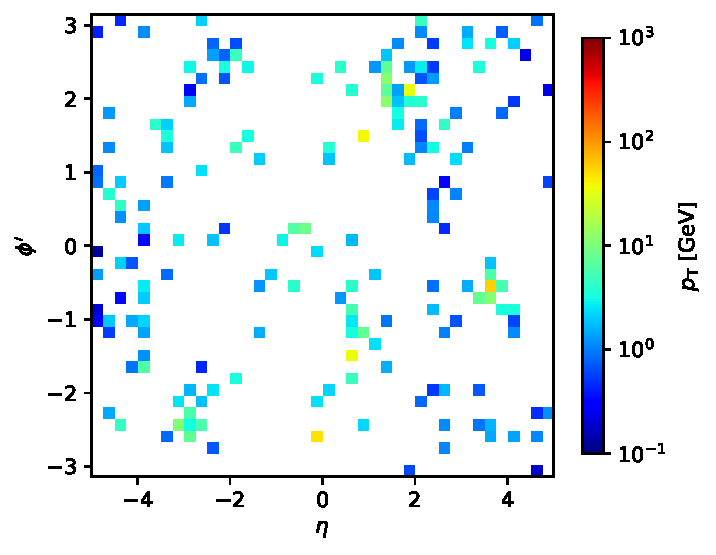
\includegraphics[width=0.45\textwidth]{event_image_GGF-ZZ_4l-tower.pdf}
            }
            \subfloat[VBF: Calorimeter Tower]{
                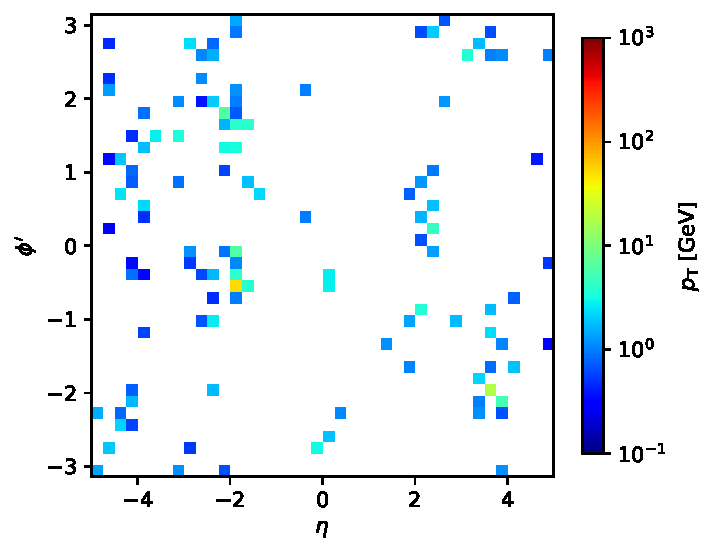
\includegraphics[width=0.45\textwidth]{event_image_VBF-ZZ_4l-tower.pdf}
            } \\
            \subfloat[GGF: Track]{
                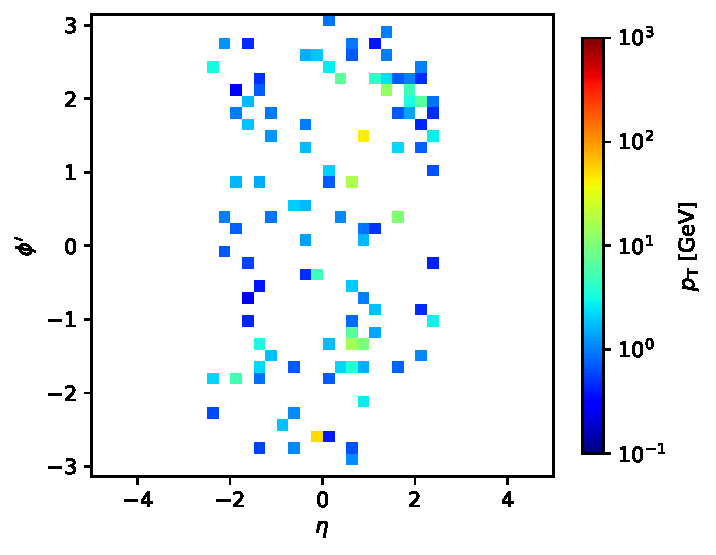
\includegraphics[width=0.45\textwidth]{event_image_GGF-ZZ_4l-track.pdf}
            }
            \subfloat[VBF: Track]{
                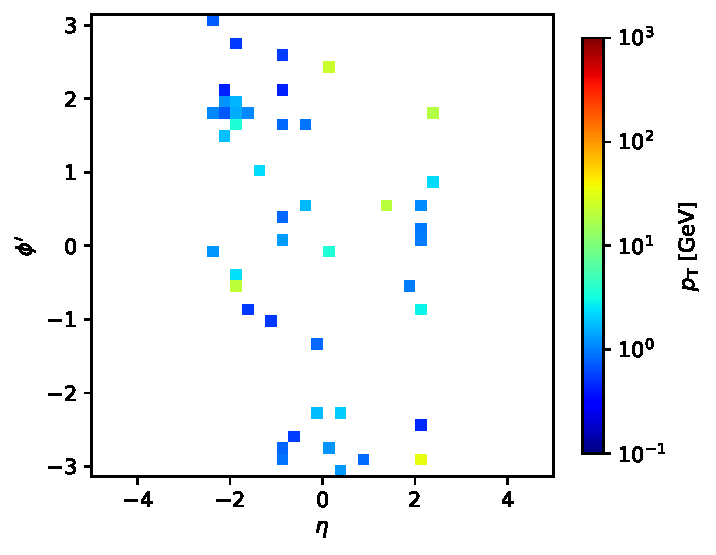
\includegraphics[width=0.45\textwidth]{event_image_VBF-ZZ_4l-track.pdf}
            } \\
            \caption{Event images for $H \to ZZ^* \to 4\ell$ events produced via GGF and VBF. Images are shown separately for the calorimeter tower and track channels.}
            \label{fig:GGF_VBF_event_image}
        \end{figure}
    % subsection event_image_of_h_to_zz_to_4ell_mode (end)
    \subsection{Testing results of di-photon classifier}% (fold)
    \label{sub:testing_results_of_di_photon_classifier}
        We evaluate the performance of the $H \to \gamma\gamma$ classifier trained in section~\ref{sec:removing_photon_information} on a different decay mode: $H \to ZZ^* \to 4\ell$. We focus on Case 1, where both the photon channel and photon-related features in the tower channel are removed from the input. This setting is designed to test whether a model trained without explicit decay production information can still extract meaningful patterns applicable to other decay modes.

        The evaluation is performed using the $2q0g$ dataset for both decay channels. Table~\ref{tab:CWoLa_CNN_training_results_3000_jet_tagging_eta_phi_aug_5_10_15_remove_photon_ZZ4l} summarizes the results.
        \begin{table}[htpb]
            \centering
            \caption{CNN training results for Case 1: both the photon channel and Tower photon-related features are removed. The classifier is trained on $H \to \gamma\gamma$ and evaluated on both $H \to \gamma\gamma$ and $H \to ZZ^* \to 4\ell$. The ACC and AUC are evaluated based on 10 training.}
            \label{tab:CWoLa_CNN_training_results_3000_jet_tagging_eta_phi_aug_5_10_15_remove_photon_ZZ4l}
            \begin{tabular}{l|cc|cc}
                         & \multicolumn{2}{c|}{$H\to\gamma\gamma$}      & \multicolumn{2}{c}{$H\to ZZ^*\to 4\ell$}           \\ \hline
                Datasets & ACC               & AUC               & ACC               & AUC               \\ \hline
                Original & $0.690 \pm 0.005$ & $0.750 \pm 0.008$ & $0.621 \pm 0.022$ & $0.665 \pm 0.027$ \\
                +5       & $0.695 \pm 0.008$ & $0.747 \pm 0.005$ & $0.592 \pm 0.012$ & $0.624 \pm 0.016$ \\
                +10      & $0.698 \pm 0.008$ & $0.752 \pm 0.010$ & $0.593 \pm 0.013$ & $0.627 \pm 0.020$ \\
                +15      & $0.700 \pm 0.010$ & $0.755 \pm 0.010$ & $0.589 \pm 0.012$ & $0.621 \pm 0.019$
            \end{tabular}
        \end{table}
        These results indicate that, although the classifier performs well on its original $H \to \gamma\gamma$ dataset, its performance degrades when applied to the $ H\to ZZ^* \to 4\ell$ events. This suggests that even after removing photon-related features, the learned representation may still carry decay-mode-specific biases that affect cross-channel transferability.
    % subsection testing_results_of_di_photon_classifier (end)
    \subsection{Testing results of supervised classifier}% (fold)
    \label{sub:testing_results_of_supervised_classifier}
		We train supervised CNN models separately on two Higgs decay channels. The training, validation, and testing dataset sizes are identical to those listed in table~\ref{tab:supervised_sample_size}. Only events that pass all selection requirements are used. Importantly, all input features directly associated with the decay products are removed.

		Table~\ref{tab:supervised_CNN_training_results_remove_product_diphoton_ZZ4l} summarizes the classification results. Each model is trained on one decay mode and evaluated on both $H \to \gamma\gamma$ and $H \to ZZ^* \to 4\ell$ datasets.
        \begin{table}[htpb]
            \centering
            \caption{CNN classification results with decay product information removed. Each model is trained on one decay channel and tested on both $H \to \gamma\gamma$ and $ H\to ZZ^* \to 4\ell$. Results are averaged over 10 training runs.}
            \label{tab:supervised_CNN_training_results_remove_product_diphoton_ZZ4l}
            \begin{tabular}{l|cc|cc}
                                     &\multicolumn{2}{c|}{$H\to\gamma\gamma$}&\multicolumn{2}{c}{$H\to ZZ^*\to 4\ell$}\\ \hline
                Training channel     & ACC               & AUC               & ACC               & AUC                \\ \hline
                $H\to\gamma\gamma$   & $0.775 \pm 0.001$ & $0.852 \pm 0.001$ & $0.752 \pm 0.002$ & $0.827 \pm 0.003$  \\
                $H\to ZZ^*\to 4\ell$ & $0.738 \pm 0.002$ & $0.806 \pm 0.003$ & $0.793 \pm 0.001$ & $0.872 \pm 0.001$ 
            \end{tabular}
        \end{table}
		Compared to the results in table~\ref{tab:supervised_CNN_training_results}, the di-photon classifier shows slightly worse performance due to the exclusion of photon-specific information.

		Although both models are trained without decay product features, the CNN still captures decay-mode-specific differences. Moreover, the model trained on $H \to ZZ^* \to 4\ell$ generalizes to the $H \to \gamma\gamma$ dataset worse than the reverse case.
    % subsection testing_results_of_supervised_classifier (end)

% section h_to_zz_to_4l_channel (end)

\section{Larger training dataset}% (fold)
\label{sec:larger_training_dataset}
    In section~\ref{sec:removing_photon_information}, we observed that removing photon information improved the training performance. There are several possible reasons for this:
    \begin{itemize}
        \item The photon channel contains large ``blank'' regions, which may confuse the neural network.
        \item Photons have higher transverse momentum, leading the network to focus on them and delay learning the jet features.
    \end{itemize}
    Increasing the size of the training dataset may mitigate these effects, allowing the network to learn both photon and jet patterns effectively.

    We evaluate model performance using the $2q0g$ dataset at different integrated luminosities, while retaining the photon information during training. The results are summarized in table~\ref{tab:CWoLa_CNN_training_results_3000_jet_tagging_L_3000_12000}.
    \begin{table}[htpb]
        \centering
        \caption{CNN training results with different dataset sizes corresponding to various luminosities. Each model is trained with photon information included. The ACC and AUC are evaluated over 10 training runs.}
        \label{tab:CWoLa_CNN_training_results_3000_jet_tagging_L_3000_12000}
        \begin{tabular}{l|cc|cc}
                                    & \multicolumn{2}{c|}{$M_1 / M_2$}      & \multicolumn{2}{c}{$S / B$}           \\ \hline
            Luminosity (fb$^{-1}$)  & ACC               & AUC               & ACC               & AUC               \\ \hline
            3000                    & $0.615 \pm 0.005$ & $0.632 \pm 0.007$ & $0.650 \pm 0.011$ & $0.703 \pm 0.015$ \\
            12000                   & $0.643 \pm 0.002$ & $0.684 \pm 0.003$ & $0.689 \pm 0.009$ & $0.743 \pm 0.011$
        \end{tabular}
    \end{table}
    These results indicate that increasing the dataset size leads to performance improvement, even when photon information is retained.
    \subsection{Logarithmic transverse momentum}% (fold)
    \label{sub:logarithmic_transverse_momentum}
        To confirm whether the high $p_{\text{T}}$ of photons affects training performance, we apply a logarithmic transformation to the $p_{\text{T}}$ values in each pixel. This aims to reduce the intensity difference between high- and low-$p_{\text{T}}$ pixels, potentially allowing the network to better focus on spatial patterns. Specifically, each pixel's input is replaced with
        \begin{equation}
            \log\left( p_{\text{T}} + 1 \right) 
        \end{equation}
        where $p_{\text{T}}$ is the original transverse momentum value. The addition of 1 takes care of $p_{\text{T}} = 0$.

        We evaluate model performance on the $2q0g$ dataset with and without the logarithmic transformation. Table~\ref{tab:CWoLa_CNN_training_results_3000_jet_tagging_log_pT} summarizes the results.
        \begin{table}[htpb]
            \centering
            \caption{CNN training results with and without the logarithmic $p_{\text{T}}$ transformation. Each model is trained with photon information included. ACC and AUC values are averaged over 10 training runs.}
            \label{tab:CWoLa_CNN_training_results_3000_jet_tagging_log_pT}
            \begin{tabular}{l|cc|cc}
                                      & \multicolumn{2}{c|}{$M_1 / M_2$}      & \multicolumn{2}{c}{$S / B$}           \\ \hline
                Dataset               & ACC               & AUC               & ACC               & AUC               \\ \hline
                Original              & $0.615 \pm 0.005$ & $0.632 \pm 0.007$ & $0.650 \pm 0.011$ & $0.703 \pm 0.015$ \\
                $\log(p_{\text{T}}) $ & $0.615 \pm 0.006$ & $0.635 \pm 0.009$ & $0.644 \pm 0.010$ & $0.694 \pm 0.014$
            \end{tabular}
        \end{table}
        The results indicate that applying the $\log(p_{\text{T}})$ transformation does not improve the performance. This suggests that intensity dominance due to high-$p_{\text{T}}$ photons may not be the main limiting factor, or that the network is already sufficiently robust to handle such variations.
    % subsection logarithmic_transverse_momentum (end)

% section larger_training_dataset (end)
\section{Event-CNN}% (fold)
\label{sec:event_cnn}
	We test an alternative network structure known as the event-CNN, as proposed in Ref.~\cite{Chiang:2022lsn}.
	\subsection{Supervised training with event-CNN}% (fold)
	\label{sub:supervised_training_with_event_cnn}
		We apply the event-CNN architecture to supervised classification tasks. The training, validation, and testing dataset sizes are identical to those listed in table~\ref{tab:supervised_sample_size}. Only events passing all selection criteria are used in training.

		Table~\ref{tab:supervised_event_CNN_training_results_diphoton} summarizes the classification performance.
        \begin{table}[htpb]
            \centering
            \caption{Event-CNN classification results. Results are averaged over 10 training runs.}
            \label{tab:supervised_event_CNN_training_results_diphoton}
            \begin{tabular}{c|c}
				 ACC               & AUC               \\ \hline
				 $0.792 \pm 0.001$ & $0.871 \pm 0.001$ \\
			\end{tabular}
        \end{table}
		Compared to the previous CNN results shown in table~\ref{tab:supervised_CNN_training_results}, the event-CNN achieves slightly better performance.
	% subsection supervised_training_with_event_cnn (end)
	\subsection{CWoLa training with event-CNN}% (fold)
	\label{sub:cwola_training_with_event_cnn}
		We consider the di-photon case mentioned in section~\ref{sec:use_jet_tagging_results_to_construct_mixed_datasets}. We also apply the $\phi$-shifting augmentation technique introduced in section~\ref{sub:phi_shifting}.
		
		Table~\ref{tab:CWoLa_event_CNN_training_results_3000_jet_tagging_phi_aug_5_10_15} summarizes the training results using the $2q0g$ dataset with $\phi$-shifting augmentation.
        \begin{table}[htpb]
            \centering
            \caption{CNN training results with different augmentation sizes. The ACC and AUC are evaluated based on 10 training.}
            \label{tab:CWoLa_event_CNN_training_results_3000_jet_tagging_phi_aug_5_10_15}
            \begin{tabular}{l|cc|cc}
                         & \multicolumn{2}{c|}{$M_1 / M_2$}      & \multicolumn{2}{c}{$S / B$}           \\ \hline
                Datasets & ACC               & AUC               & ACC               & AUC               \\ \hline
                Original & $0.624 \pm 0.011$ & $0.644 \pm 0.021$ & $0.679 \pm 0.009$ & $0.739 \pm 0.012$ \\
                +5       & $0.649 \pm 0.004$ & $0.691 \pm 0.005$ & $0.681 \pm 0.005$ & $0.739 \pm 0.005$ \\
                +10      & $0.650 \pm 0.004$ & $0.692 \pm 0.004$ & $0.678 \pm 0.007$ & $0.735 \pm 0.010$ \\
                +15      & $0.651 \pm 0.004$ & $0.694 \pm 0.005$ & $0.676 \pm 0.006$ & $0.732 \pm 0.007$
            \end{tabular}
        \end{table}
		Although $\phi$-shifting improves model performance on mixed datasets, the enhancement saturates as the dataset size increases. Notably, on pure samples, the performance remains similar regardless of augmentation, indicating that the gain is primarily due to over-fitting on mixed datasets.
	% subsection cwola_training_with_event_cnn (end)
    \subsection{Remove photon information with event-CNN}% (fold)
    \label{sub:remove_photon_information_with_event_cnn}
        To investigate the role of photon inputs in training, we apply the event-CNN model to the Case 1 datasets described in section~\ref{sec:removing_photon_information}.

        We use the $2q0g$ datasets for evaluation. The training results are summarized in table~\ref{tab:CWoLa_event_CNN_training_results_3000_jet_tagging_eta_phi_case1}.
        \begin{table}[htpb]
            \centering
            \caption{Event-CNN training results with both the photon channel and Tower photon features removed (Case 1). The ACC and AUC are evaluated based on 10 training.}
            \label{tab:CWoLa_event_CNN_training_results_3000_jet_tagging_eta_phi_case1}
            \begin{tabular}{l|cc|cc}
                         & \multicolumn{2}{c|}{$M_1 / M_2$}      & \multicolumn{2}{c}{$S / B$}           \\ \hline
                Datasets & ACC               & AUC               & ACC               & AUC               \\ \hline
                Original & $0.624 \pm 0.011$ & $0.644 \pm 0.021$ & $0.679 \pm 0.009$ & $0.739 \pm 0.012$ \\
                Case 1   & $0.637 \pm 0.012$ & $0.667 \pm 0.020$ & $0.682 \pm 0.004$ & $0.740 \pm 0.005$ \\
            \end{tabular}
        \end{table}
        The training performance is almost the same, suggesting that the model can still extract discriminative features from the jet pattern alone.
    % subsection remove_photon_information_with_event_cnn (end)
    \subsection{Various training size with event-CNN}% (fold)
    \label{sub:various_training_size_with_event_cnn}
        We also study the effect of dataset size on the model's performance. The event-CNN is trained using the $2q0g$ datasets corresponding to different integrated luminosities, while keeping photon information included. The results are summarized in table~\ref{tab:CWoLa_event_CNN_training_results_jet_tagging_various_L}.
        \begin{table}[htpb]
            \centering
            \caption{Event-CNN training results with different dataset sizes corresponding to various luminosities. Each model is trained with photon information included. The ACC and AUC are evaluated over 10 training runs.}
            \label{tab:CWoLa_event_CNN_training_results_jet_tagging_various_L}
            \begin{tabular}{l|cc|cc}
                                        & \multicolumn{2}{c|}{$M_1 / M_2$}      & \multicolumn{2}{c}{$S / B$}           \\ \hline
                Luminosity (fb$^{-1}$)  & ACC               & AUC               & ACC               & AUC               \\ \hline
                300                     & $0.610 \pm 0.015$ & $0.589 \pm 0.036$ & $0.606 \pm 0.033$ & $0.641 \pm 0.045$ \\
                900                     & $0.625 \pm 0.007$ & $0.628 \pm 0.009$ & $0.660 \pm 0.014$ & $0.715 \pm 0.018$ \\
                1800                    & $0.625 \pm 0.010$ & $0.644 \pm 0.019$ & $0.674 \pm 0.009$ & $0.732 \pm 0.012$ \\
                3000                    & $0.624 \pm 0.011$ & $0.644 \pm 0.021$ & $0.679 \pm 0.009$ & $0.739 \pm 0.012$ \\
                12000                   & $0.655 \pm 0.002$ & $0.701 \pm 0.003$ & $0.683 \pm 0.004$ & $0.742 \pm 0.005$
            \end{tabular}
        \end{table}
        The performance improved with increased dataset size. For the pure datasets, the training performance is saturated after $3000 \text{ fb}^{-1}$.

        We repeat the analysis using datasets where photon information has been removed. The comparison between the two scenarios is shown in figure~\ref{fig:eventCNN_AUC_various_L}. In the high-luminosity regime, the model performance is similar regardless of whether photon information is included. However, at lower luminosities, datasets without photon information unexpectedly yield better AUC.
        \begin{figure}[htpb]
            \centering
            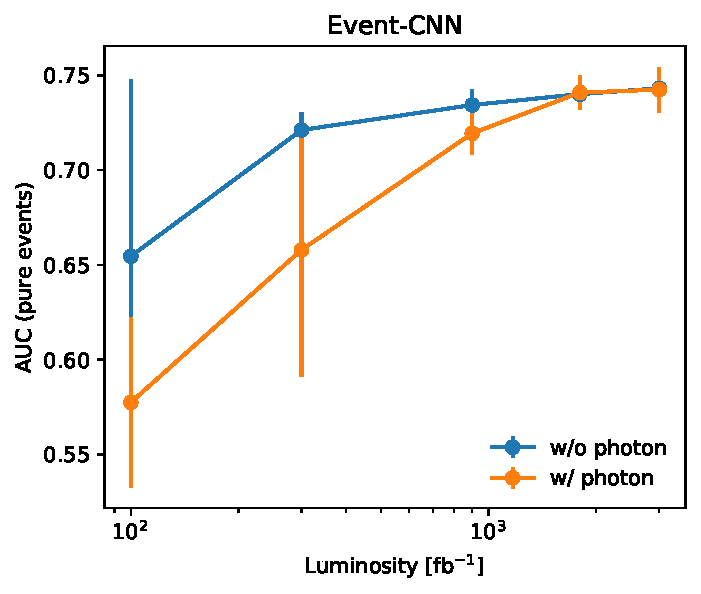
\includegraphics[width=0.60\textwidth]{event_CNN_AUC-true_L.pdf}
            \caption{AUC comparison for Event-CNN models trained with and without photon information across different luminosities. The average and standard deviation are evaluated over 10 training runs.}
            \label{fig:eventCNN_AUC_various_L}
        \end{figure}
    % subsection various_training_size_with_event_cnn (end)
    \subsection{Photon information removed datasets with \texorpdfstring{$\phi$}{phi}-shifting augmentation}% (fold)
    \label{sub:photon_information_removed_datasets_with_phi_shifting_augmentation}
        We test the $\phi$-shifting augmentation of the photon information removed case. Here, we consider the luminosity of $\mathcal{L} = \text{100 fb}^{-1}$.
        
        Table~\ref{tab:CWoLa_event_CNN_training_results_100_jet_tagging_phi_aug_5_10_15} summarizes the training results using the $2q0g$ dataset with $\phi$-shifting augmentation.
        \begin{table}[htpb]
            \centering
            \caption{Event-CNN training results for the photon-removed dataset with different $\phi$-shifting augmentation sizes. ACC and AUC are averaged over 10 training runs.}
            \label{tab:CWoLa_event_CNN_training_results_100_jet_tagging_phi_aug_5_10_15}
            \begin{tabular}{l|cc|cc}
                         & \multicolumn{2}{c|}{$M_1 / M_2$}      & \multicolumn{2}{c}{$S / B$}           \\ \hline
                Datasets & ACC               & AUC               & ACC               & AUC               \\ \hline
                Original & $0.627 \pm 0.028$ & $0.601 \pm 0.066$ & $0.617 \pm 0.064$ & $0.655 \pm 0.093$ \\
                +5       & $0.623 \pm 0.017$ & $0.621 \pm 0.036$ & $0.657 \pm 0.019$ & $0.709 \pm 0.024$ \\
                +10      & $0.627 \pm 0.018$ & $0.634 \pm 0.033$ & $0.663 \pm 0.011$ & $0.718 \pm 0.015$ \\
                +15      & $0.627 \pm 0.016$ & $0.635 \pm 0.034$ & $0.660 \pm 0.009$ & $0.713 \pm 0.011$
            \end{tabular}
        \end{table}
        The results show that $\phi$-shifting augmentation improves model performance. The $\phi$-shifting augmentation helps mitigate statistical fluctuations and improve generalization.
    % subsection photon_information_removed_datasets_with_phi_shifting_augmentation (end)
    \subsection{\texorpdfstring{$H \to ZZ^* \to 4\ell$}{H to ZZ to 4l} channel}% (fold)
    \label{sub:h_to_zz_to_4l_channel}
        We follow the same setup as described in section~\ref{sec:h_to_zz_to_4l_channel}. For CWoLa training, we consider multiple luminosity scenarios. In the case of $\mathcal{L} = \text{3000 fb}^{-1}$, the number of events in the mixed datasets is shown in table~\ref{tab:number_of_event_in_mixed_dataset_gluon_jet_ZZ4l}.
        
        The event-CNN training results are summarized in table~\ref{tab:CWoLa_event_CNN_training_results_jet_tagging_ZZ4l_L_3000_30000}. At $\mathcal{L} = \text{3000 fb}^{-1}$, the ACC and AUC are close to 0.5, indicating that the training is nearly ineffective. However, as the training dataset size increases to $\mathcal{L} = \text{30000 fb}^{-1}$, the AUC for the pure dataset improves significantly, reaching values around 0.8. This highlights the importance of dataset size.
        \begin{table}[htpb]
            \centering
            \caption{Event-CNN training results using datasets corresponding to different luminosities. The $ZZ \to 4\ell$ decay channel is considered, with information on the decay products included. ACC and AUC are averaged over 10 training runs.}
            \label{tab:CWoLa_event_CNN_training_results_jet_tagging_ZZ4l_L_3000_30000}
            \begin{tabular}{l|cc|cc}
                                        & \multicolumn{2}{c|}{$M_1 / M_2$}      & \multicolumn{2}{c}{$S / B$}           \\ \hline
                Luminosity (fb$^{-1}$)  & ACC               & AUC               & ACC               & AUC               \\ \hline
                3000                    & $0.575 \pm 0.012$ & $0.508 \pm 0.039$ & $0.538 \pm 0.026$ & $0.543 \pm 0.035$ \\
                30000                   & $0.601 \pm 0.010$ & $0.621 \pm 0.012$ & $0.732 \pm 0.018$ & $0.800 \pm 0.023$
            \end{tabular}
        \end{table}

        To assess the contribution of decay products to model performance, we train the event-CNN on the $\mathcal{L} = \text{30000 fb}^{-1}$ dataset with all lepton-related information removed. Since lepton signals can appear in both Tower and Track channels, we mask the corresponding pixels by setting them to zero in both inputs. The results are shown in table~\ref{tab:CWoLa_event_CNN_training_results_30000_jet_tagging_ZZ4l_case5}.
        \begin{table}[htpb]
            \centering
            \caption{Event-CNN training results after removing all decay product information. ACC and AUC are averaged over 10 training runs.}
            \label{tab:CWoLa_event_CNN_training_results_30000_jet_tagging_ZZ4l_case5}
            \begin{tabular}{l|cc|cc}
                           & \multicolumn{2}{c|}{$M_1 / M_2$}      & \multicolumn{2}{c}{$S / B$}           \\ \hline
                Datasets   & ACC               & AUC               & ACC               & AUC               \\ \hline
                Original   & $0.601 \pm 0.010$ & $0.621 \pm 0.012$ & $0.732 \pm 0.018$ & $0.800 \pm 0.023$ \\
                w/o lepton & $0.606 \pm 0.010$ & $0.626 \pm 0.012$ & $0.645 \pm 0.006$ & $0.697 \pm 0.009$
            \end{tabular}
        \end{table}
        The performance is 10\% worse for pure events when lepton information is removed, indicating that some of the discriminative features are removed.

        We apply the event-CNN model trained on the photon-removed $H \to \gamma\gamma$ dataset (from section~\ref{sub:photon_information_removed_datasets_with_phi_shifting_augmentation}) to $H \to ZZ^* \to 4\ell$ events. The evaluation uses the $2q0g$ datasets for both decay channels, and the results are summarized in table~\ref{tab:CWoLa_event_CNN_training_results_100_jet_tagging_phi_aug_5_10_15_remove_photon_ZZ4l}.
        \begin{table}[htpb]
            \centering
            \caption{Event-CNN training results for phton-removed datasets. The classifier is trained on $H \to \gamma\gamma$ and evaluated on both $H \to \gamma\gamma$ and $H \to ZZ^* \to 4\ell$. The ACC and AUC are evaluated based on 10 training.}
            \label{tab:CWoLa_event_CNN_training_results_100_jet_tagging_phi_aug_5_10_15_remove_photon_ZZ4l}
            \begin{tabular}{l|cc|cc}
                         &\multicolumn{2}{c|}{$H\to\gamma\gamma$}&\multicolumn{2}{c}{$H\to ZZ^*\to4\ell$}\\ \hline
                Datasets & ACC               & AUC               & ACC               & AUC               \\ \hline
                Original & $0.617 \pm 0.061$ & $0.655 \pm 0.089$ & $0.599 \pm 0.041$ & $0.634 \pm 0.056$ \\
                +5       & $0.663 \pm 0.015$ & $0.717 \pm 0.020$ & $0.634 \pm 0.015$ & $0.677 \pm 0.018$ \\
                +10      & $0.667 \pm 0.010$ & $0.723 \pm 0.014$ & $0.638 \pm 0.010$ & $0.683 \pm 0.011$ \\
                +15      & $0.664 \pm 0.009$ & $0.719 \pm 0.010$ & $0.634 \pm 0.006$ & $0.679 \pm 0.009$
            \end{tabular}
        \end{table}
        These results demonstrate the transferability of the event-CNN model across decay channels. The AUC for $ZZ \to 4\ell$ is comparable to that achieved by training directly on $ZZ \to 4\ell$ events at $\mathcal{L} = 30000~\text{fb}^{-1}$.

        This suggests that, by leveraging both dataset augmentation and transfer learning, we can effectively simulate the performance equivalent to having approximately 29900~fb$^{-1}$ of additional data. This approach offers a practical path to improving tagger performance in channels with limited statistics.
    % subsection h_to_zz_to_4l_channel (end)
    \subsection{Supervised learning without photon information}% (fold)
    \label{sub:supervised_learning_without_photon_information}
        We perform the supervised training of the event-CNN without photon information to explore the importance of the photon-related features.

        Table~\ref{tab:supervised_event_CNN_training_results_diphoton_w_wo_photon} and figure~\ref{fig:eventCNN_roc_curve} summarize the training results. 
        \begin{table}[htpb]
            \centering
            \caption{Event-CNN classification results. Results are averaged over 10 training runs. The 10 training runs use the same dataset, only the initial weights are different.}
            \label{tab:supervised_event_CNN_training_results_diphoton_w_wo_photon}
            \begin{tabular}{c|cc}
                 Datasets  & ACC               & AUC               \\ \hline
                 w/ photon & $0.792 \pm 0.001$ & $0.871 \pm 0.001$ \\
                 w/o photon & $0.784 \pm 0.001$ & $0.862 \pm 0.001$ \\
			\end{tabular}
        \end{table}
        The event-CNN achieves slightly better performance when photon information is included. However, the small difference in AUC indicates that the model is still able to extract meaningful features from the jet pattern.
        \begin{figure}[htpb]
            \centering
            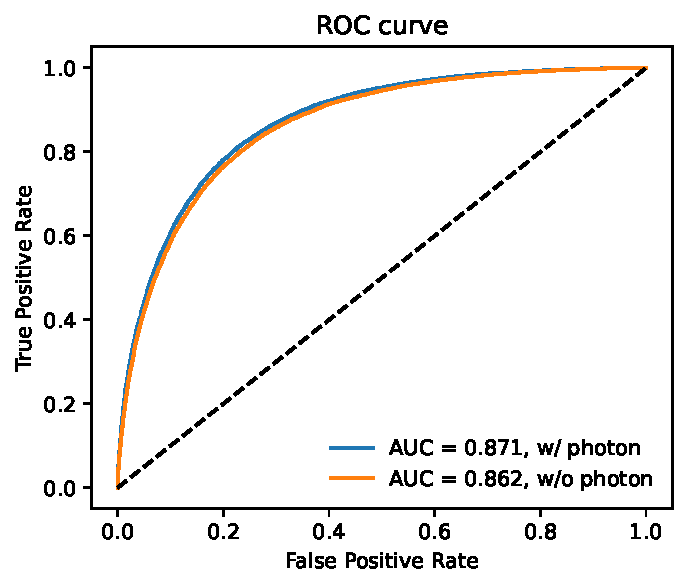
\includegraphics[width=0.60\textwidth]{roc_curve_supervised.pdf}
            \caption{ROC curves for event-CNN models trained with and without photon information.}
            \label{fig:eventCNN_roc_curve}
        \end{figure}
    % subsection supervised_learning_without_photon_information (end)
% section event_cnn (end)
\section{Particle transformer}% (fold)
\label{sec:particle_transformer}
	We test an alternative network structure known as the Particle Transformer (ParT), as proposed in Ref.~\cite{Qu:2022mxj}.
    \subsection{Supervised training with ParT}% (fold)
    \label{sub:supervised_training_with_part}
        We apply the ParT architecture to supervised classification tasks. The training, validation, and testing dataset sizes are identical to those listed in table~\ref{tab:supervised_sample_size}. Only events passing all selection criteria are used in training.

		Table~\ref{tab:supervised_ParT_training_results} summarizes the training results. 
        \begin{table}[htpb]
            \centering
            \caption{ParT classification results. Results are averaged over 10 training runs. The 10 training runs use the same dataset, only the initial weights are different.}
            \label{tab:supervised_ParT_training_results}
            \begin{tabular}{c|cc}
                 Datasets  & ACC               & AUC               \\ \hline
                 w/ photon & $0.785 \pm 0.013$ & $0.862 \pm 0.014$ \\
                 w/o photon & $0.773 \pm 0.019$ & $0.850 \pm 0.022$ \\
			\end{tabular}
        \end{table}
        % \begin{figure}[htpb]
        %     \centering
        %     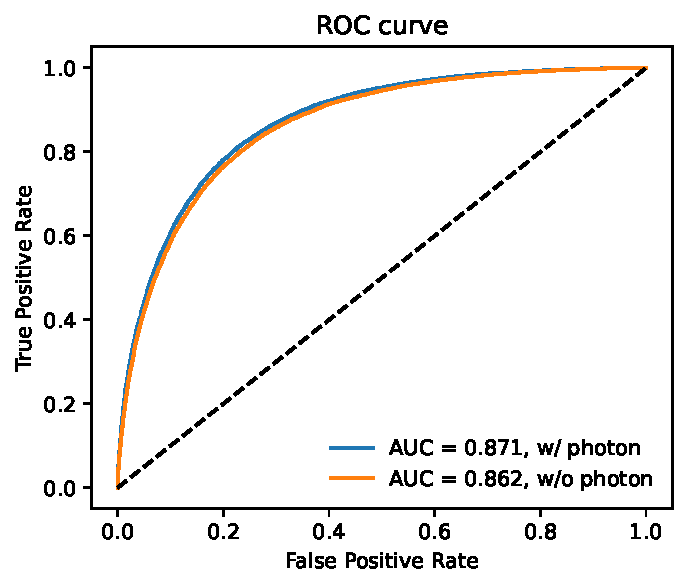
\includegraphics[width=0.60\textwidth]{roc_curve_supervised.pdf}
        %     \caption{ROC curves for ParT models trained with and without photon information.}
        %     \label{fig:supervised_ParT_roc_curve}
        % \end{figure}
		Compared to the previous results shown in table~\ref{tab:supervised_event_CNN_training_results_diphoton_w_wo_photon} for event-CNN architecture, the ParT achieves slightly worse performance.
    % subsection supervised_training_with_part (end)
    \subsection{CWoLa training with ParT}% (fold)
    \label{sub:cwola_training_with_part}
        We also study the effect of dataset size on the model's performance. The ParT is trained using the $2q0g$ datasets corresponding to different integrated luminosities. Table~\ref{tab:CWoLa_ParT_training_results_jet_tagging_various_L} summarizes the training results with and without photon information.
        \begin{table}[htpb]
            \centering
            \caption{ParT training results with different dataset sizes corresponding to various luminosities. The ACC and AUC are evaluated over 10 training runs.}
            \label{tab:CWoLa_ParT_training_results_jet_tagging_various_L}
            \subfloat[With photon]{
                \begin{tabular}{l|cc|cc}
                                            & \multicolumn{2}{c|}{$M_1 / M_2$}      & \multicolumn{2}{c}{$S / B$}           \\ \hline
                    Luminosity (fb$^{-1}$)  & ACC               & AUC               & ACC               & AUC               \\ \hline
                    100                     & $0.603 \pm 0.015$ & $0.539 \pm 0.041$ & $0.544 \pm 0.043$ & $0.540 \pm 0.078$ \\
                    300                     & $0.607 \pm 0.015$ & $0.549 \pm 0.066$ & $0.572 \pm 0.071$ & $0.584 \pm 0.112$ \\
                    900                     & $0.620 \pm 0.013$ & $0.617 \pm 0.060$ & $0.657 \pm 0.062$ & $0.705 \pm 0.099$ \\
                    1800                    & $0.609 \pm 0.018$ & $0.575 \pm 0.071$ & $0.607 \pm 0.086$ & $0.638 \pm 0.117$ \\
                    3000                    & $0.622 \pm 0.019$ & $0.607 \pm 0.088$ & $0.648 \pm 0.097$ & $0.681 \pm 0.152$ \\
                \end{tabular}
            } \\
            \subfloat[Without photon]{
                \begin{tabular}{l|cc|cc}
                                            & \multicolumn{2}{c|}{$M_1 / M_2$}      & \multicolumn{2}{c}{$S / B$}           \\ \hline
                    Luminosity (fb$^{-1}$)  & ACC               & AUC               & ACC               & AUC               \\ \hline
                    100                     & $0.612 \pm 0.019$ & $0.544 \pm 0.061$ & $0.545 \pm 0.044$ & $0.536 \pm 0.082$ \\
                    300                     & $0.602 \pm 0.012$ & $0.535 \pm 0.062$ & $0.556 \pm 0.046$ & $0.564 \pm 0.072$ \\
                    900                     & $0.610 \pm 0.020$ & $0.576 \pm 0.064$ & $0.595 \pm 0.080$ & $0.625 \pm 0.110$ \\
                    1800                    & $0.620 \pm 0.022$ & $0.592 \pm 0.098$ & $0.637 \pm 0.105$ & $0.661 \pm 0.168$ \\
                    3000                    & $0.637 \pm 0.008$ & $0.667 \pm 0.015$ & $0.714 \pm 0.022$ & $0.782 \pm 0.026$ \\
                \end{tabular}
            }
        \end{table}

        The comparison between the two scenarios is shown in figure~\ref{fig:ParT_AUC_various_L}. The training performance is very unstable in both cases. Some trainings have totally failed.
        \begin{figure}[htpb]
            \centering
            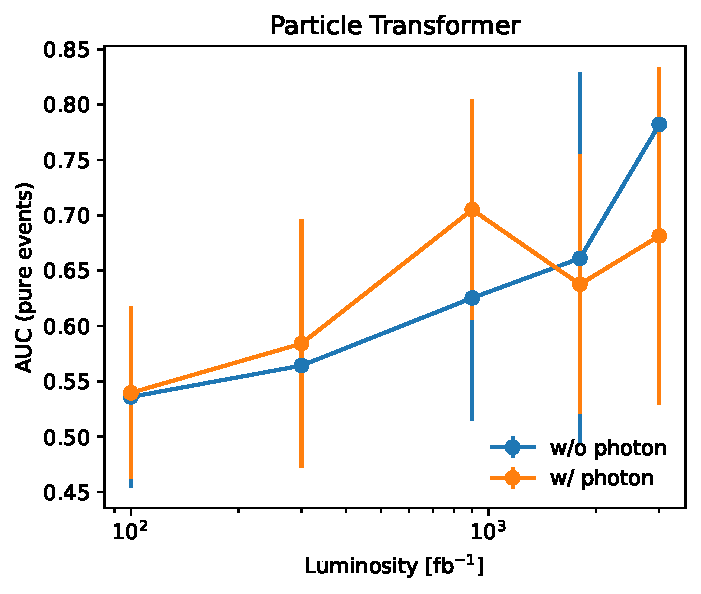
\includegraphics[width=0.60\textwidth]{ParT_AUC-true_L.pdf}
            \caption{AUC comparison for ParT models trained with and without photon information across different luminosities. The average and standard deviation are evaluated over 10 training runs.}
            \label{fig:ParT_AUC_various_L}
        \end{figure}
    % subsection cwola_training_with_part (end)
    \subsection{\texorpdfstring{$\phi$}{phi}-shifting augmentation on ParT}% (fold)
    \label{sub:phi_shifting_augmentation_on_part}
        We test the $\phi$-shifting augmentation of the photon information removed case. Here, we consider the luminosity of $\mathcal{L} = \text{100 fb}^{-1}$.
        
        Table~\ref{tab:CWoLa_ParT_training_results_100_jet_tagging_phi_aug_5_10_15} summarizes the training results using the $2q0g$ dataset with $\phi$-shifting augmentation.
        \begin{table}[htpb]
            \centering
            \caption{ParT training results for the photon-removed dataset with different $\phi$-shifting augmentation sizes. ACC and AUC are averaged over 10 training runs.}
            \label{tab:CWoLa_ParT_training_results_100_jet_tagging_phi_aug_5_10_15}
            \begin{tabular}{l|cc|cc}
                         & \multicolumn{2}{c|}{$M_1 / M_2$}      & \multicolumn{2}{c}{$S / B$}           \\ \hline
                Datasets & ACC               & AUC               & ACC               & AUC               \\ \hline
                Original & $0.612 \pm 0.019$ & $0.544 \pm 0.061$ & $0.545 \pm 0.044$ & $0.536 \pm 0.082$ \\
                +5       & $0.595 \pm 0.005$ & $0.495 \pm 0.031$ & $0.515 \pm 0.014$ & $0.492 \pm 0.042$ \\
                +10      & $0.606 \pm 0.017$ & $0.552 \pm 0.065$ & $0.579 \pm 0.063$ & $0.599 \pm 0.094$ \\
                +15      & $0.630 \pm 0.028$ & $0.620 \pm 0.065$ & $0.646 \pm 0.066$ & $0.693 \pm 0.093$
            \end{tabular}
        \end{table}
        The results show that $\phi$-shifting augmentation improves model performance. The $\phi$-shifting augmentation helps improve generalization, but can not mitigate the statistical fluctuation.
    % subsection phi_shifting_augmentation_on_part (end)
    \subsection{Implementing \texorpdfstring{$p_{\mathrm{T}}$}{pT} normalization with ParT}% (fold)
    \label{sub:implement_pt_normalization_with_part}
        We apply $p_{\text{T}}$ normalization to investigate whether it can mitigate training fluctuations. The ParT model is trained on the $2q0g$ datasets corresponding to different integrated luminosities.

        The comparison between the two setups is shown in figure~\ref{fig:ParT_AUC_various_L_pTnorm}. In both cases, the training performance remains unstable, and in some runs, the training completely fails.
        \begin{figure}[htpb]
            \centering
            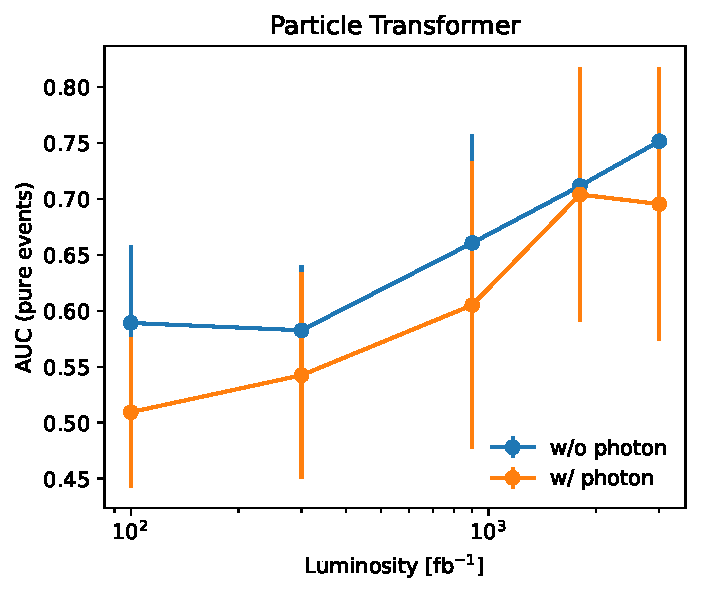
\includegraphics[width=0.60\textwidth]{ParT_AUC-true_L-pTnorm.pdf}
            \caption{AUC comparison for ParT models trained with $p_{\text{T}}$ normalization across different luminosities. The average and standard deviation are evaluated over 10 independent training runs.}
            \label{fig:ParT_AUC_various_L_pTnorm}
        \end{figure}
    % subsection implement_pt_normalization_with_part (end)
    \subsection{Implementing a learning rate schedule}% (fold)
    \label{sub:implement_learning_rate_schedule}

        We introduce a learning rate schedule with a warm-up to prevent the training from diverging in the early stage. The schedule combines a short warm-up phase with a subsequent exponential decay strategy. The ParT model is trained on the $2q0g$ datasets corresponding to different integrated luminosities.

        The comparison between the two scenarios is shown in figure~\ref{fig:ParT_AUC_various_L_pTnorm_lr_schedule}. The training performance still exhibits instabilities, but the completely failed cases are fewer than in previous testing.
        \begin{figure}[htpb]
            \centering
            % 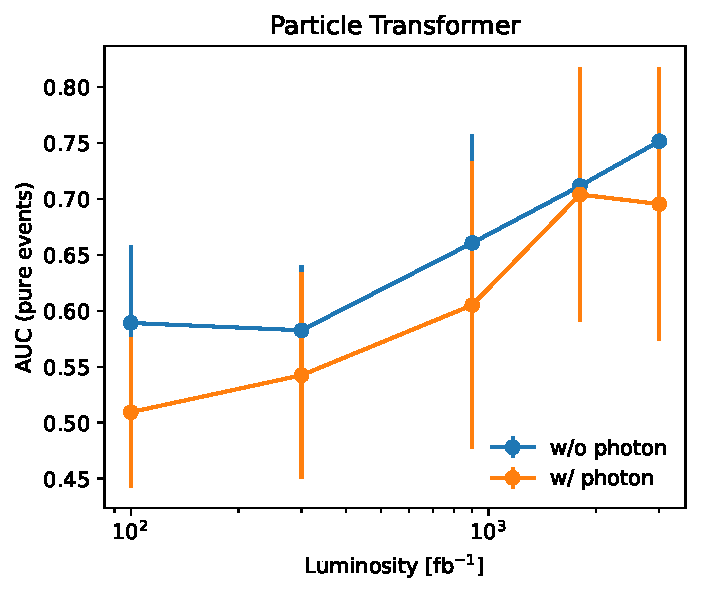
\includegraphics[width=0.60\textwidth]{ParT_AUC-true_L-pTnorm.pdf}
            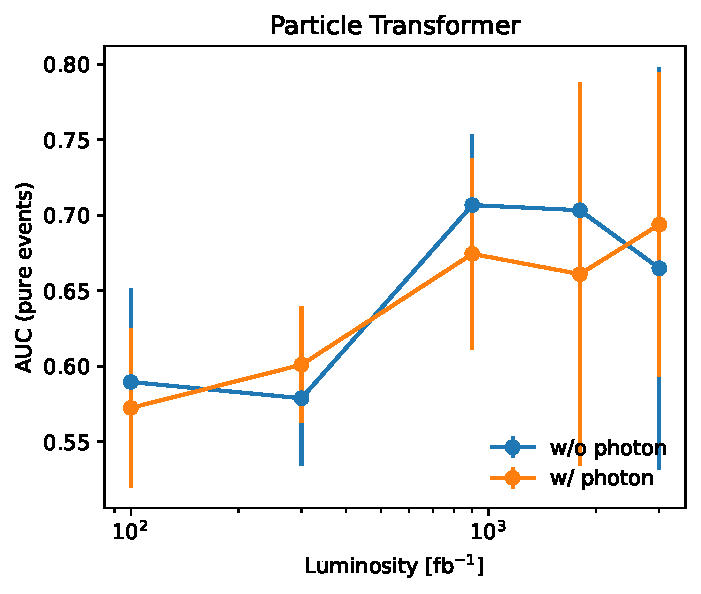
\includegraphics[width=0.60\textwidth]{ParT_AUC-true_L-pTnorm_lr_schedule.pdf}
            \caption{AUC comparison for ParT models trained with learning rate schedule across different luminosities. The average and standard deviation are evaluated over 10 independent training runs.}
            \label{fig:ParT_AUC_various_L_pTnorm_lr_schedule}
        \end{figure}
    % subsection implement_learning_rate_schedule (end)

% section particle_transformer (end)
\section{Comparison of training sample}% (fold)
\label{sec:comparison_of_training_sample}
    There are some differences between Yian's and my training sample preparation workflows:
    \begin{enumerate}
        \item Yian did not apply flipping.
        \item For the $\phi$-translation, I computed a common $\phi$-center for all channels, while Yian computed the $\phi$-center for each channel separately.
    \end{enumerate}
    It is not immediately clear how these differences affect the training results. To investigate this, I tested supervised and CWoLa training on event-CNN using Yian's samples.

    For the supervised training, we used the same setup as in section~\ref{sub:supervised_training_with_event_cnn}. Table~\ref{tab:supervised_event_CNN_training_results_diphoton_w_wo_photon_yian_sample} summarizes the classification performance. 
    \begin{table}[htpb]
        \centering
        \caption{Event-CNN classification results using Yian's and FY's samples. Results are averaged over 10 training runs.}
        \label{tab:supervised_event_CNN_training_results_diphoton_w_wo_photon_yian_sample}
        \begin{tabular}{c|cc|cc}
            Datasets   & \multicolumn{2}{c|}{Yian}             & \multicolumn{2}{c}{FY}                \\ \hline
                       & ACC               & AUC               & ACC               & AUC               \\ \hline
            w/ photon  & $0.782 \pm 0.001$ & $0.859 \pm 0.001$ & $0.792 \pm 0.001$ & $0.871 \pm 0.001$ \\
            w/o photon & $0.781 \pm 0.001$ & $0.858 \pm 0.001$ & $0.784 \pm 0.001$ & $0.862 \pm 0.001$
        \end{tabular}
    \end{table}
    Yian's results are worse than FY's by about 1\% for the photon case.

    For CWoLa training, we trained models with different luminosities. Table~\ref{tab:CWoLa_eventCNN_training_results_jet_tagging_various_L_yian} summarizes the results with and without photon information.  
    \begin{table}[htpb]
        \centering
        \caption{Event-CNN training results using Yian's samples with different dataset sizes corresponding to various luminosities. Results are averaged over 10 training runs.}
        \label{tab:CWoLa_eventCNN_training_results_jet_tagging_various_L_yian}
        \subfloat[With photon]{
            \begin{tabular}{l|cc|cc}
                                        & \multicolumn{2}{c|}{$M_1 / M_2$}      & \multicolumn{2}{c}{$S / B$}           \\ \hline
                Luminosity (fb$^{-1}$)  & ACC               & AUC               & ACC               & AUC               \\ \hline
                100                     & $0.604 \pm 0.017$ & $0.517 \pm 0.054$ & $0.560 \pm 0.046$ & $0.572 \pm 0.074$ \\
                300                     & $0.603 \pm 0.009$ & $0.585 \pm 0.021$ & $0.620 \pm 0.006$ & $0.662 \pm 0.009$ \\
                900                     & $0.609 \pm 0.006$ & $0.606 \pm 0.011$ & $0.640 \pm 0.005$ & $0.694 \pm 0.007$ \\
                1800                    & $0.609 \pm 0.006$ & $0.616 \pm 0.013$ & $0.652 \pm 0.011$ & $0.708 \pm 0.015$ \\
                3000                    & $0.615 \pm 0.005$ & $0.630 \pm 0.012$ & $0.665 \pm 0.015$ & $0.724 \pm 0.018$ \\
            \end{tabular}
        } \\
        \subfloat[Without photon]{
            \begin{tabular}{l|cc|cc}
                                        & \multicolumn{2}{c|}{$M_1 / M_2$}      & \multicolumn{2}{c}{$S / B$}           \\ \hline
                Luminosity (fb$^{-1}$)  & ACC               & AUC               & ACC               & AUC               \\ \hline
                100                     & $0.608 \pm 0.023$ & $0.541 \pm 0.069$ & $0.553 \pm 0.039$ & $0.563 \pm 0.061$ \\
                300                     & $0.607 \pm 0.009$ & $0.590 \pm 0.026$ & $0.610 \pm 0.024$ & $0.651 \pm 0.034$ \\
                900                     & $0.611 \pm 0.005$ & $0.612 \pm 0.012$ & $0.637 \pm 0.009$ & $0.691 \pm 0.011$ \\
                1800                    & $0.611 \pm 0.007$ & $0.619 \pm 0.013$ & $0.656 \pm 0.017$ & $0.712 \pm 0.021$ \\
                3000                    & $0.620 \pm 0.009$ & $0.640 \pm 0.018$ & $0.669 \pm 0.016$ & $0.728 \pm 0.020$ \\
            \end{tabular}
        }
    \end{table}

    The comparison among different cases is shown in figure~\ref{fig:eventCNN_AUC_various_L_yian_FY}. Overall, Yian's results are worse than FY's. These results suggest that differences in the sample preparation workflow have a direct impact on the training performance.  
    \begin{figure}[htpb]
        \centering
        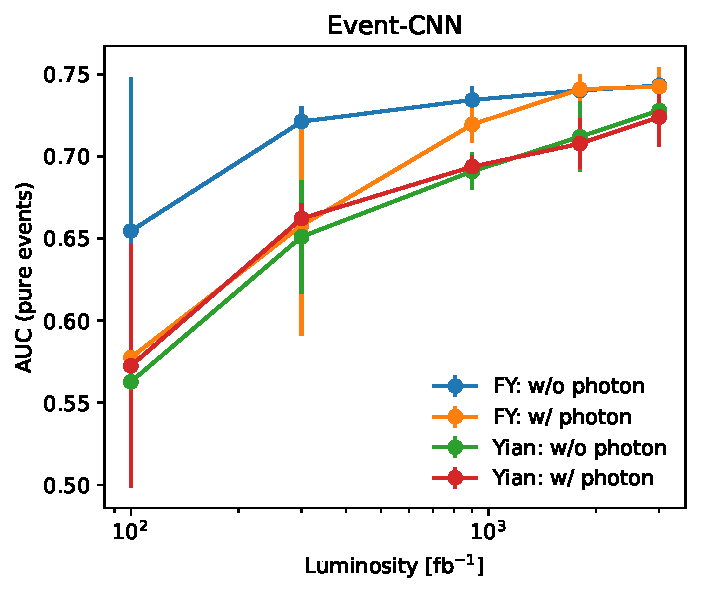
\includegraphics[width=0.60\textwidth]{event_CNN_AUC-true_L_yian_FY.pdf}
        \caption{AUC comparison for event-CNN models trained with and without photon information across different luminosities. Results are averaged over 10 training runs, with error bars indicating standard deviations.}
        \label{fig:eventCNN_AUC_various_L_yian_FY}
    \end{figure}

    The following step is included for Yian's pre-processing flow:
    \begin{itemize}
        \item another moving in the $\phi$-direction. This moves to ensure the high intensity $p_{\text{T}}$ region does not cross the $\pm\pi$ boundary.
    \end{itemize}

    The comparison among different cases is shown in figure~\ref{fig:eventCNN_AUC_various_L_yian0905_FY}. Overall, Yian's results are consistent than FY's. The main differences are the without photon case in low luminosities.  
    \begin{figure}[htpb]
        \centering
        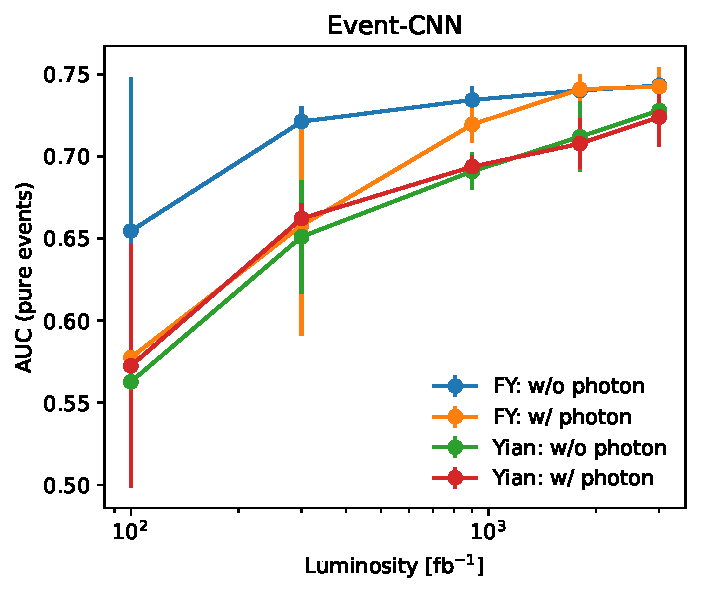
\includegraphics[width=0.60\textwidth]{event_CNN_AUC-true_L_yian_FY.pdf}
        % \includegraphics[width=0.60\textwidth]{event_CNN_AUC-true_L_yian0905_FY.pdf}
        \caption{AUC comparison for event-CNN models trained with and without photon information across different luminosities. Results are averaged over 10 training runs, with error bars indicating standard deviations.}
        \label{fig:eventCNN_AUC_various_L_yian0905_FY}
    \end{figure}
% section comparison_of_training_sample (end)

\section{Modify the training setup for Transformer}% (fold)
\label{sec:modify_the_training_setup_for_transformer}
    The training results of the Transformer model are highly unstable in my setup, a behavior not observed in Yian’s training. To investigate the possible cause, we compared the pre-processed datasets. The inputs for the with and without photon cases yield almost identical values after preprocessing, suggesting that the instability is not due to discrepancies in the input samples.

    In the comparison, we unexpectedly found that roughly 0.1\% VBF events contain no constituents in the TRACK channel. Since the Particle Transformer can handle NaN values, we do not expect this issue to be the primary cause of the training failures.

    We further tested a range of hyperparameter configurations, varying the batch size from 128 to 512 and the learning rate from $10^{-5}$ to $4\times10^{-4}$. However, all of these setups still resulted in unstable training, with the runs failing.

    Finally, we found that this issue stems from the ``logit output.'' The logit refers to the raw classifier output before applying a normalization function such as sigmoid or softmax. In my original setup, the loss function did not correctly account for this, leading to inconsistent optimization behavior. The recommended usage is to specify \verb|from_logits=True| in the \texttt{BinaryCrossentropy} function, as shown below:
    \begin{verbatim}
        model.compile(
            loss=keras.losses.BinaryCrossentropy(from_logits=True),
            ...
        )
    \end{verbatim}
    After fixing this issue, the training process became much more stable. Figure~\ref{fig:ParT_AUC_various_L_pTnorm_logit} presents the updated results. In both the with- and without-photon cases, the models now exhibit consistent training behavior, and no completely failed runs are observed.
    \begin{figure}[htpb]
        \centering
        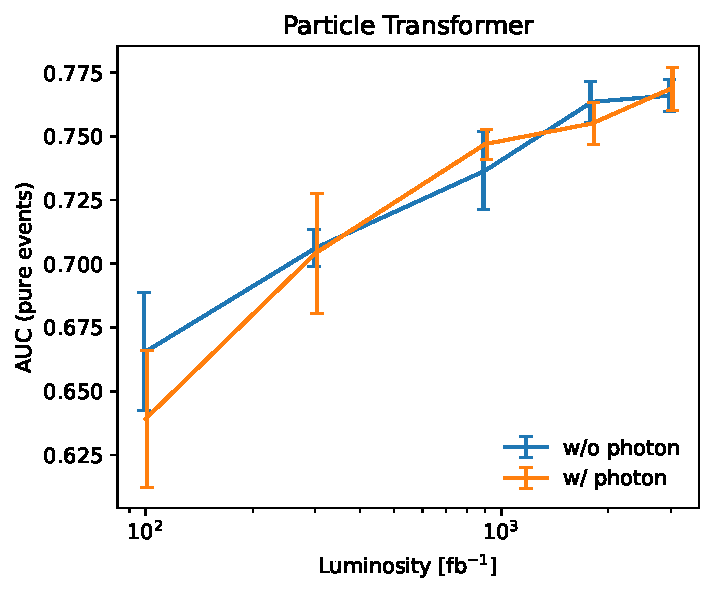
\includegraphics[width=0.60\textwidth]{ParT_AUC-true_L-pTnorm_logit.pdf}
        \caption{AUC comparison for ParT models trained with $p_{\text{T}}$ normalization across different luminosities. Results are averaged over 10 independent training runs, with error bars indicating standard deviations.}
        \label{fig:ParT_AUC_various_L_pTnorm_logit}
    \end{figure}
% section modify_the_training_setup_for_transformer (end)

\bibliographystyle{ieeetr}
\bibliography{reference}

\end{document}
